% !TEX program = xelatex
% =============================================================================
% Block Round --- 教学设计 (zh-CN)
% 面向中国大陆高三（普通高中三年级）的5课时教学序列，
% 锚定 Minecraft 我的世界（国服：网易我的世界）。
% 视觉风格与 docs_math/Block_Round_Math_zh-CN.pdf 保持一致。
% 编译：xelatex Plano_de_Aula_zh-CN.tex （两次以生成目录与交叉引用）
% =============================================================================
\documentclass[12pt,a4paper]{scrartcl}

% ---------- 字体（与 docs_math/Block_Round_Math_zh-CN.tex 一致） ----------
\usepackage{fontspec}
\usepackage{xeCJK}
\setCJKmainfont{Microsoft YaHei}[Scale=1.05]
\setCJKsansfont{Microsoft YaHei}[Scale=1.05]
\setmainfont{Latin Modern Roman}[Scale=1.05]
\setsansfont{Latin Modern Sans}[Scale=1.05]
\setmonofont{Latin Modern Mono}
\usepackage{unicode-math}
\setmathfont{Latin Modern Math}[Scale=1.05]

% ---------- 宏包 ----------
\usepackage{amsmath}
\usepackage{mathtools}

\usepackage[a4paper,top=2.8cm,bottom=2.8cm,left=2.6cm,right=2.6cm,
            headheight=16pt]{geometry}
\usepackage{microtype}
\usepackage{xcolor}
\usepackage{booktabs}
\usepackage{array}
\usepackage{tabularx}
\usepackage{enumitem}
\usepackage{titlesec}
\usepackage{fancyhdr}
\usepackage{graphicx}
\usepackage{csquotes}
\usepackage{tcolorbox}
\tcbuselibrary{skins,breakable}
\usepackage{needspace}
\usepackage{caption}
\usepackage{subcaption}
\usepackage{float}

\raggedbottom

% ---------- Block Round 色板 ----------
\definecolor{accent}{HTML}{5B8E3F}      % Minecraft 草地绿
\definecolor{accentdark}{HTML}{406A2A}
\definecolor{earth}{HTML}{825432}        % 泥土棕
\definecolor{ink}{HTML}{1F1F23}
\definecolor{muted}{HTML}{4E4E58}
\definecolor{bg}{HTML}{FBF6E9}
\definecolor{rule}{HTML}{D8D1BC}
\definecolor{linkc}{HTML}{2D5A1F}        % 链接深绿

\usepackage[colorlinks=true,
            linkcolor=linkc,
            urlcolor=linkc,
            citecolor=linkc,
            breaklinks=true,
            bookmarks=true,bookmarksopen=true,
            pdftitle={Block Round --- 教学设计 (zh-CN)},
            pdfauthor={Vinicius Rodrigues de Souza}]{hyperref}
\usepackage{xurl}

\color{ink}

\widowpenalty=10000
\clubpenalty=10000

% ---------- 章节样式 ----------
\titleformat{\section}
  {\sffamily\Large\bfseries\color{accent}}{\thesection.}{0.6em}{}
\titleformat{\subsection}
  {\sffamily\large\bfseries\color{accent!85!ink}}{\thesubsection}{0.6em}{}
\titleformat{\subsubsection}
  {\sffamily\normalsize\bfseries\color{muted}}{\thesubsubsection}{0.5em}{}
\titlespacing*{\section}{0pt}{1.2\baselineskip}{0.6\baselineskip}
\titlespacing*{\subsection}{0pt}{0.8\baselineskip}{0.3\baselineskip}
\titlespacing*{\subsubsection}{0pt}{0.6\baselineskip}{0.2\baselineskip}

% ---------- 页眉页脚 ----------
\pagestyle{fancy}
\fancyhf{}
\fancyhead[L]{\small\sffamily\bfseries\color{accent}BLOCK ROUND}
\fancyhead[R]{\small\sffamily\color{muted}教学设计 --- 高三}
\fancyfoot[L]{\small\sffamily\color{muted}Block Round --- 教学资料}
\fancyfoot[R]{\small\sffamily\color{muted}第 \thepage{} 页}
\renewcommand{\headrulewidth}{0.4pt}
\renewcommand{\footrulewidth}{0.4pt}
\renewcommand{\headrule}{{\color{rule}\hrule height \headrulewidth}}
\renewcommand{\footrule}{{\color{rule}\vskip-\footrulewidth\hrule height \footrulewidth\vskip-\footrulewidth}}

% ---------- 教学盒子 ----------
% 环境名必须使用 ASCII；标题用中文。
\newtcolorbox{gongshi}{
  colback=bg, colframe=rule, boxrule=0.4pt, arc=2pt,
  left=10pt,right=10pt,top=8pt,bottom=8pt,
  before skip=8pt, after skip=8pt,
  fontupper=\color{accentdark}, breakable,
  before={\par\needspace{4\baselineskip}}
}

\newtcolorbox{huodong}[1][活动]{
  enhanced, breakable,
  colback=bg, colframe=accent, boxrule=0.6pt, arc=4pt,
  left=12pt,right=12pt,top=10pt,bottom=10pt,
  before skip=12pt, after skip=12pt,
  before={\par\needspace{5\baselineskip}},
  attach boxed title to top left={xshift=10pt,yshift=-8pt},
  boxed title style={colback=accent,colframe=accent,boxrule=0pt,arc=2pt},
  coltitle=white, fonttitle=\sffamily\bfseries\small,
  title=#1
}

\newtcolorbox{zhushi}[1][教学札记]{
  enhanced, breakable,
  colback=bg!50!white, colframe=rule, boxrule=0.4pt, arc=2pt,
  left=10pt,right=10pt,top=8pt,bottom=8pt,
  before skip=8pt, after skip=8pt,
  before={\par\needspace{3\baselineskip}},
  attach boxed title to top left={xshift=10pt,yshift=-7pt},
  boxed title style={colback=muted,colframe=muted,boxrule=0pt,arc=2pt},
  coltitle=white, fonttitle=\sffamily\bfseries\footnotesize,
  title=#1
}

\newtcolorbox{biaozhun}[1][课标要求]{
  enhanced,
  breakable=false,
  colback=bg!70!white, colframe=accent!60!ink, boxrule=0.4pt, arc=2pt,
  left=10pt,right=10pt,top=6pt,bottom=6pt,
  before skip=6pt, after skip=6pt,
  before={\par\needspace{8\baselineskip}},
  attach boxed title to top left={xshift=10pt,yshift=-6pt},
  boxed title style={colback=accent!60!ink,colframe=accent!60!ink,boxrule=0pt,arc=2pt},
  coltitle=white, fonttitle=\sffamily\bfseries\footnotesize,
  title=#1
}

\newtcolorbox{minecraft}[1][我的世界]{
  enhanced, breakable,
  colback=accent!7, colframe=earth!70!accent, boxrule=0.5pt, arc=3pt,
  left=10pt,right=10pt,top=8pt,bottom=8pt,
  before skip=10pt, after skip=10pt,
  before={\par\needspace{3\baselineskip}},
  attach boxed title to top left={xshift=10pt,yshift=-7pt},
  boxed title style={colback=earth,colframe=earth,boxrule=0pt,arc=2pt},
  coltitle=white, fonttitle=\sffamily\bfseries\footnotesize,
  title=#1
}

\setlength{\parskip}{0.75em}
\setlength{\parindent}{0pt}
\linespread{1.10}

\setlength{\textfloatsep}{14pt plus 2pt minus 2pt}
\setlength{\floatsep}{14pt plus 2pt minus 2pt}
\setlength{\intextsep}{14pt plus 2pt minus 2pt}

\captionsetup{font=small, labelfont={bf,color=accent}, textfont={color=muted}, justification=centering}
\captionsetup[sub]{font=footnotesize, labelfont={bf,color=accent!75!ink}, textfont={color=muted}}

\graphicspath{{img/}}

\newcommand{\code}[1]{\texttt{\small #1}}
\newcommand{\acc}[1]{\textcolor{accent}{\textbf{#1}}}
\newcommand{\cmd}[1]{\textcolor{earth}{\texttt{\small #1}}}
\newcommand{\tempo}[1]{\textnormal{\footnotesize\color{bg!90!white}\textsf{#1}}}

\begin{document}

% =============================================================================
% 封面
% =============================================================================
\begin{titlepage}
  \centering
  \vspace*{3.0cm}
  {\sffamily\bfseries\fontsize{56}{60}\selectfont \color{accent} Block Round\par}
  \vspace{0.7cm}
  {\sffamily\LARGE\color{muted} 教学设计\par}
  \vspace{0.25cm}
  {\sffamily\Large\color{muted} 普通高中三年级（高三）\par}
  \vspace{1.0cm}
  {\color{rule}\rule{0.6\textwidth}{0.6pt}\par}
  \vspace{0.7cm}
  \begin{minipage}{0.84\textwidth}
    \centering\color{ink}\large
    面向中国大陆普通高中三年级学生的5课时教学序列，
    引入 \emph{Block Round} 体素生成器。围绕同一个核心问题——
    \emph{如何在有限的方块网格上表示连续曲线，并如何将该表示转化为
    青少年最熟悉的文化载体——我的世界（Minecraft）中可建造的结构}——
    将\emph{解析几何}、\emph{计算思维}、\emph{信息技术核心素养}
    与\emph{我的世界建造实践}有机融合。
  \end{minipage}
  \vspace{0.7cm}\\
  {\color{rule}\rule{0.6\textwidth}{0.6pt}\par}
  \vspace{0.9cm}
  \begin{minipage}{0.78\textwidth}
    \centering
    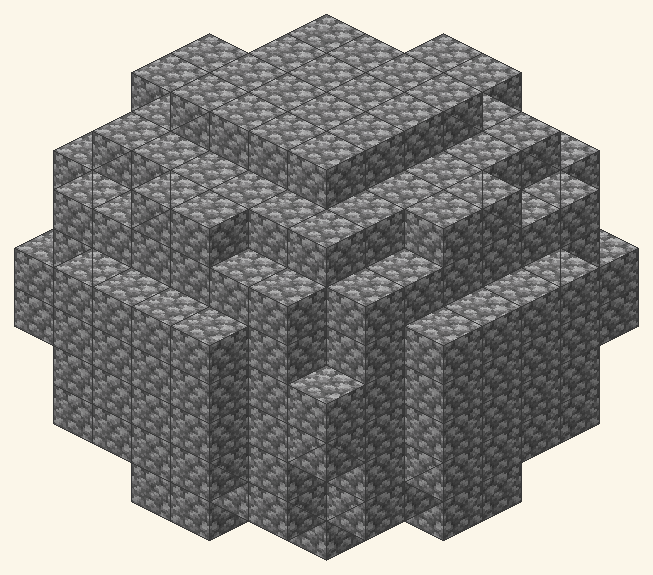
\includegraphics[width=0.55\linewidth]{fig10_3d_sphere_d12.png}\\[0.4em]
    {\sffamily\footnotesize\color{muted}直径10的球被 Block Round 体素化，使用我的世界 \emph{cobblestone}（圆石）贴图渲染。}
  \end{minipage}
  \vspace{0.7cm}\\
  {\color{rule}\rule{0.6\textwidth}{0.6pt}\par}
  \vspace{0.9cm}
  \begin{minipage}{0.82\textwidth}
    \centering\sffamily\small\color{muted}
    \textbf{融合学科：}数学 $\cdot$ 语文/艺术（数字艺术、设计）$\cdot$ 信息技术 $\cdot$ 通用技术 $\cdot$ 游戏化学习 \\[0.4em]
    \textbf{对接标准：}《普通高中数学课程标准（2017年版2020年修订）》$\cdot$ 新高考改革 $\cdot$ 高考数学 $\cdot$ \hyperref[sec:obmep]{高中数学联赛 / 信息学奥赛} $\cdot$ Minecraft Education（国服：网易我的世界）
  \end{minipage}
\end{titlepage}

% =============================================================================
\renewcommand{\contentsname}{\color{accent}目录}
\tableofcontents
\thispagestyle{fancy}
\newpage

% =============================================================================
\section{基本信息与背景}\label{sec:identificacao}

\begin{center}
\begin{tabular}{@{}p{0.32\textwidth}p{0.62\textwidth}@{}}
\toprule
\textbf{学科} & 数学（与艺术、信息技术、通用技术、历史、地理高度融合）。\\
\addlinespace[2pt]
\textbf{学段与年级} & 普通高中三年级（高三）。可下移用于高二，亦可用于成人高中、国家开放大学的预科衔接班。\\
\addlinespace[2pt]
\textbf{适用类型} & 普通高中（重点/示范/普通），中等职业学校的"中职+三 二/三 三"分流前、国际部（IB/AP/A-Level），民族中学双语班，乡镇高中，成人高中、夜校或函授班。\\
\addlinespace[2pt]
\textbf{课时安排} & 5 课时 $\times$ 50 分钟（共计 250 分钟课堂时间）$+$ 可选课外延展活动。100 分钟"大课"合并模式见 §\ref{sec:adapt}。\\
\addlinespace[2pt]
\textbf{核心资源} & Block Round —— 免费\emph{网页}应用，无需注册、无服务器、浏览器中可离线运行（PWA）。符合《个人信息保护法》（PIPL）：不采集、不上传任何个人信息。可在低端\emph{智能手机}上流畅运行 —— 无需 Java，无需安装我的世界客户端。\\
\addlinespace[2pt]
\textbf{课标主题} & 必修课程主题三 \emph{几何与代数}（直线方程、圆的方程、空间向量、立体几何）$\cdot$ 选择性必修主题二 \emph{圆锥曲线}（椭圆、双曲线、抛物线）$\cdot$ 信息技术核心素养。\\
\addlinespace[2pt]
\textbf{六大核心素养} & 数学抽象 $\cdot$ 逻辑推理 $\cdot$ 数学建模 $\cdot$ 直观想象 $\cdot$ 数学运算 $\cdot$ 数据分析。本教学序列同时调动这六项。\\
\addlinespace[2pt]
\textbf{选修方向衔接} & \emph{数学拓展}（数学建模、数学探究活动）；可与\emph{信息技术}课程的算法与程序设计模块联动；适用于\emph{综合实践活动}与\emph{研究性学习}课时。\\
\addlinespace[2pt]
\textbf{学习路径关联} & \hyperref[sec:obmep]{全国高中数学联赛}（CMO 省赛） $\cdot$ 全国青少年信息学奥赛 NOIP/NOI $\cdot$ \emph{强基计划}数学方向 $\cdot$ \emph{丘成桐少年班} $\cdot$ Minecraft Education（国服 \emph{网易我的世界}）。\\
\addlinespace[2pt]
\textbf{学生先备知识} & 平面直角坐标系；圆的标准方程（高一）；基本几何体的面积与体积（高二）；函数的概念；比例与百分比。我的世界使用经验（建议但非强制；\emph{Block Round} 本身不要求）。\\
\addlinespace[2pt]
\textbf{教师课前准备} & 20分钟 Block Round 自主探索；阅读 \texttt{docs\_math/Block\_Round\_Math\_zh-CN.pdf}（中文技术文档）；选学：我的世界 Java版 命令 \cmd{/fill}、\cmd{/clone}、\cmd{//sphere} 的基础用法。\\
\bottomrule
\end{tabular}
\end{center}

\begin{zhushi}[中国大陆高中的多样性]
本教学序列面向中国大陆高中教育的多样性场景：北京四中、上海中学、人大附中、华东师大二附中、广州执信、深圳实验、北师大实验中学等一线/二线城市的重点中学；三四线/地级市的省级示范高中；中等职业学校、国际部（IB/AP/A-Level）；县乡级乡镇普通高中；蒙古族、藏族、维吾尔族、朝鲜族、回族、壮族等少数民族中学（按《民族区域自治法》设立的民族类双语学校）；新疆喀什、西藏拉萨、内蒙古呼和浩特、广西南宁、云南德宏、青海玉树等地的边远地区中学；以及成人高中、国家开放大学、网络远程教育（电大）的成人学习者。每种场景对应不同的调整方案，统一汇总于 §\ref{sec:adapt}。Block Round 被选为核心工具的根本原因是它\emph{适应上述所有场景}：可在低端\emph{智能手机}上运行，首次加载后无需联网（PWA），不需注册、不需身份证号、不采集任何个人信息——这是《个人信息保护法》的硬性要求。
\end{zhushi}

\begin{minecraft}[为什么以"我的世界"为锚点]
《我的世界》（Minecraft）是历史上销量最高的电子游戏（全球累计超过 3 亿份）。在中国，网易自 2017 年起获得 Mojang 授权运营国服\emph{网易我的世界}（NetEase Minecraft），月活跃用户超过 1 亿，其中相当比例为中学生。哔哩哔哩（B站）上抽风Crazy\_、Joe粥、锐刻五Reek\_、籽岷ZeMin、小宝Babyfu 等知名 UP 主拥有上百万订阅。在中国互联网络信息中心（CNNIC）与中国信息通信研究院（CAICT）发布的青少年游戏行为报告中，《我的世界》始终位列中学生最常游玩的游戏前三名，跨越东中西部、城乡、收入差异。\emph{以"我的世界"为教学锚点不是赶时髦——而是承认：中国青少年早已在那里"做几何"。}
\end{minecraft}

% =============================================================================
\section{教学立意与理论依据}\label{sec:justificativa}

将 Block Round 作为高三数学教学的核心工具，是对当代中国基础教育\acc{五重诉求}的综合回应：把形式化的数学与信息技术核心素养有机融合（\emph{2017年版2020年修订课标}强调的"信息技术与数学课程整合"）；让抽象知识扎根于学生\emph{有意义的}日常实践；备战高考全国卷中圆与圆锥曲线、立体几何（球的体积与表面积）的命题趋势；衔接\emph{新高考改革}（"3+1+2"或"3+3"模式下的数学选考与综合考察）；以及在不损失数学严谨性的前提下，借助\emph{我的世界}这一最普及的青少年文化载体作为学习动机的桥梁。

\emph{体素艺术}（voxel art）已成为中国当代青少年的文化常识。\emph{我的世界}——2009年诞生，2014年被微软以25亿美元收购，今天通过\emph{Minecraft Education}（中国大陆由网易代理）走入校园——是中国中学生中跨地域、跨城乡、跨阶层的文化共识。把"以方块建造"作为教学起点，等于把一个\emph{游戏化的}熟悉传统转化为\emph{真正的数学问题}：在 $1 \times 1 \times 1$ 的离散方块网格上，描述由 $\mathbb{R}^3$ 上解析定义的连续形体。每天在国服服务器上建造立方体、塔楼、圆形农场、穹顶的学生会突然意识到：他凭直觉做的事情有正式的名字——\emph{体素化}、\emph{离散光栅化}、\emph{椭球的隐式方程}。

本教学举动与中国教育的\emph{五条传统}相呼应：

\begin{itemize}[leftmargin=1.3em,itemsep=0.2em,topsep=0.3em]
  \item \acc{孔子}（公元前551--479，《论语》：\emph{因材施教}、\emph{温故而知新}、\emph{学而不思则罔}）。东方教育以学生本人的认识起点为起点，本序列正是从学生已经在游戏里"建造圆球"的经验出发，而非从形式化方程出发——这是因材施教在数字时代的体现。

  \item \acc{陶行知}（1891--1946，"生活即教育"、"教学做合一"、"小先生制"）。陶先生的思想与本序列高度契合：建造、试错、与同学讨论、再优化，正是\emph{教学做合一}的现代版本。我的世界把"做"——learning by doing——推到极致：玩家实时检验自己的建造假设。

  \item \acc{蔡元培}（1868--1940，北京大学校长，"思想自由、兼容并包"、"以美育代宗教"）。蔡元培强调艺术与科学并重；本序列正是在数学课堂里同时进行美学决策（贴图选择）与数学推理（算法选择）。

  \item \acc{张奠宙、顾明远}与中国数学教育现代化。张奠宙先生（华东师范大学，《数学教育学导论》）系统奠定中国数学教育的现代理论基础；顾明远先生（北京师范大学，比较教育与教师专业发展）推动了课程与教学的国际比较。本序列在数学建模、信息技术整合的理念上，承袭这一脉络。

  \item \acc{民族数学（ethnomathematics）的中国视角}。乌比拉坦·杜安布罗西奥（D'Ambrosio）的民族数学理论被译介进入中国（张维忠等学者，北京师范大学）。Block Round 中的三个算法（\emph{欧几里得 / Bresenham / 阈值}）可读作"对同一个问题的三种民族数学解法"；而中国玩家在 B站发布的圆球建造教程构成第四种——\emph{当代}的、\emph{口语}的、\emph{游戏中介的}本土民族数学。
\end{itemize}

软件在此承担明确的认识论功能：\emph{它不替代}代数推导，而是\emph{把数学定义之间的差异变得可见}。三个算法对应对同一对象——\emph{离散圆周}——的三种数学定义，并产生肉眼可分辨的不同图形（图\ref{fig:comp-d10}）。学生用\emph{眼睛}看到："定义不同结果就不同"，并同时意识到结果不是抽象的——\emph{他能在我的世界里把它一砖一块地建起来}。

\begin{figure}[!htbp]
\centering
\begin{subfigure}[t]{0.31\linewidth}\centering
  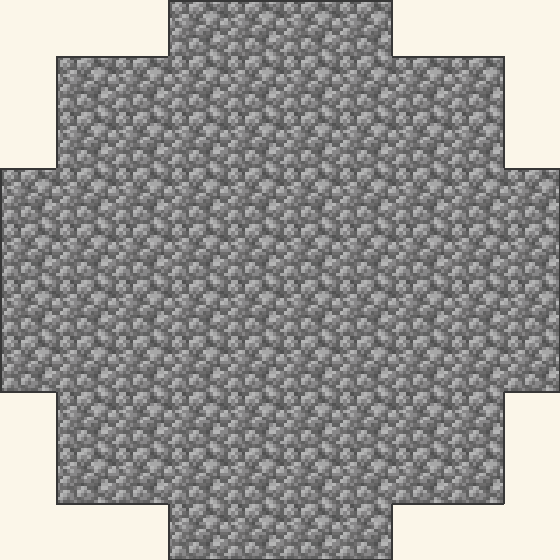
\includegraphics[width=\linewidth]{fig01_2d_d10_euclidean.png}
  \caption{\emph{欧几里得}}
\end{subfigure}\hfill
\begin{subfigure}[t]{0.31\linewidth}\centering
  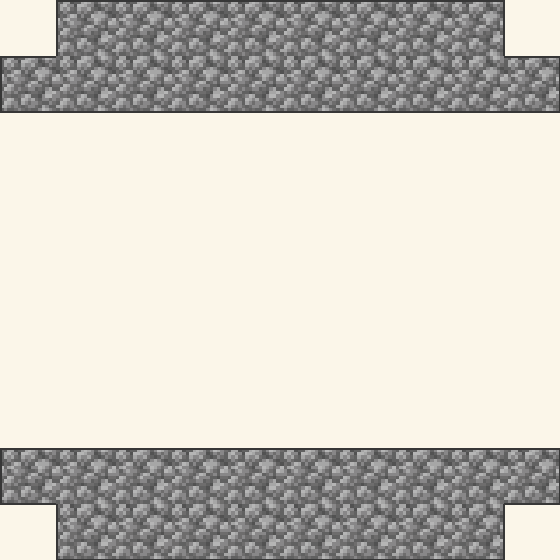
\includegraphics[width=\linewidth]{fig02_2d_d10_bresenham.png}
  \caption{\emph{Bresenham}}
\end{subfigure}\hfill
\begin{subfigure}[t]{0.31\linewidth}\centering
  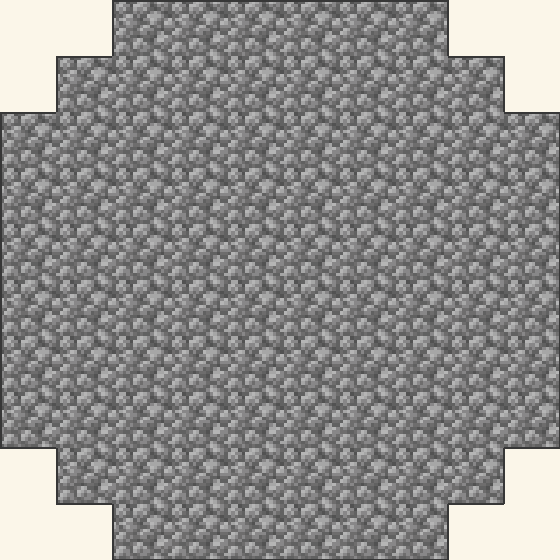
\includegraphics[width=\linewidth]{fig03_2d_d10_threshold.png}
  \caption{\emph{阈值}}
\end{subfigure}
\caption{同一直径10的圆，在三种不同的"属于判据"下的体素化结果，使用我的世界 \emph{cobblestone}（圆石）贴图。注意四角格、行间过渡、四个基本方位上的差异——它们是三种\emph{数学上都正确}的方案，对应我的世界中的三种不同建造图纸。}
\label{fig:comp-d10}
\end{figure}

\begin{zhushi}[公平性与中国基础教育的资源现实]
Block Round 的选择也回应了一个具体的资源公平问题：中国大陆基础教育资源的地区差异。教育部教育统计数据显示，2023年东部沿海地区高中信息技术机房配备率显著高于西部省份，山区与县乡学校的设备老化更新滞后。但同期 PNAD 类统计（CNNIC 中学生网络使用调查）显示，普通智能手机在 15--17 岁青少年中的拥有率超过 90\%，覆盖东中西部。Block Round 正是为这一现实而设计：可在 2018 年以来的低价 Android 手机上流畅运行，无需持续联网（PWA），不需注册——而当学校连手机都不允许时，附录~\ref{ap:adapt-analog} 提供了完全\emph{纸质}的版本。\emph{我的世界基岩版（Pocket Edition）即便在三年旧的国产手机上也能运行}——学生可以在课堂用 Block Round 起步，回家在我的世界国服延续。
\end{zhushi}

\begin{minecraft}[研究：我的世界在中国基础教育中的应用]
近年来，中国研究者发表了多篇关于《我的世界》在教育中的应用研究：华东师范大学、北京师范大学、首都师范大学等师范院校的教育技术系发表了若干硕士论文与期刊论文，讨论 Minecraft 在编程教育、几何教学、跨学科项目学习中的应用；网易我的世界教育版官方网站（\url{https://edu.163.com/mc}）维护中文教学方案与教师培训计划；教育部"国家中小学智慧教育平台"中已有若干基于游戏化的数学课例。本教学序列以 Block Round 为\emph{桥梁}：在不安装游戏（即不需 Java、不需账号、不依赖国服注册流程）的情况下，让我的世界的几何思维进入课堂。
\end{minecraft}

% =============================================================================
\section{教学目标}\label{sec:objetivos}

\subsection{总目标}

引导学生\acc{理解、比较、运用并转化为建造行动}圆、椭圆与椭球的形式定义，将其作为在体素化方块网格上判断方格"属于"或"不属于"的判据；调用这些图形的隐式方程来\emph{解释、预测、修改并在我的世界中建造}具有原创性的视觉作品；同时与中华文化几何遗产（青铜器纹饰、苏州园林漏窗、客家土楼、良渚玉琮、北京天坛、国家大剧院、故宫太和殿屋脊曲线）以及中国数学传统对话。这种"多种正确解"的意识与中国当代数学的国际地位相呼应：1982 年丘成桐（华裔）获菲尔兹奖、2006 年陶哲轩（华裔）获菲尔兹奖、2013 年张益唐在孪生素数猜想上取得突破性进展。同时与一种当代的中国玩家文化对话——B站、哔哩哔哩、网易我的世界国服上，玩家社群每天都在不自觉地\emph{做}空间几何。

\subsection{具体目标}

\textbf{认知目标（概念性）：}
\begin{itemize}[leftmargin=1.3em,itemsep=0.2em,topsep=0.3em]
  \item 把椭圆的隐式方程 $\left(\dfrac{x}{r_x}\right)^{\!2} + \left(\dfrac{y}{r_y}\right)^{\!2} = 1$ 识别为含圆 $x^2 + y^2 = r^2$ 的一般情形；
  \item 认识到三种不同的"属于判据"（中心点距离、Bresenham 中点判断、角点覆盖）产生三个不同的方格集合——如图~\ref{fig:comp-d10} 所示；
  \item 理解 2D 方程到 3D 椭球方程的推广，并将其与球体积公式 $V = \tfrac{4}{3}\pi r_x r_y r_z$ 联系起来（高考全国卷立体几何高频考点）；
  \item 把空间中的一个平面对体的切割解读为对体素中心点坐标的\emph{线性不等式}；
  \item 理解\emph{我的世界的物品栏算术}（64 个方块为一组 stack，单箱27格，双箱54格）作为\emph{除法取整}与\emph{商与余数表示}的具体应用；
  \item 识别构造一个完整球体所需的\emph{对称}（反射、旋转），并将其用于 \cmd{/clone} 命令的优化建造。
\end{itemize}

\textbf{操作目标（程序性）：}
\begin{itemize}[leftmargin=1.3em,itemsep=0.2em,topsep=0.3em]
  \item 在 Block Round 中切换 2D 与 3D 模式，导出 PNG 图像与 \texttt{.schem} 蓝图文件；
  \item 在坐标纸上手工绘制圆的离散近似，应用欧几里得判据，并与软件输出对比；
  \item 通过\emph{数格子}计算体素化图形的离散面积/体积，并与连续面积/体积比较，表示相对误差；
  \item 将圆、椭圆、椭球组合为原创作品，并以数学依据为每项选择辩护；同时预估各类方块所需数量与双箱数；
  \item 在 Litematica 或 Schematica 模组中导入 Block Round 导出的 \texttt{.schem}，并在我的世界游戏内执行建造；
  \item 编写一组 \cmd{/clone} 命令序列，将"一个八分之一象限"对称扩展为完整球体。
\end{itemize}

\textbf{情感与态度目标：}
\begin{itemize}[leftmargin=1.3em,itemsep=0.2em,topsep=0.3em]
  \item 以双人或三人小组形式协作完成实践活动，模拟我的世界服务器中的\emph{builders} 团队工作模式；
  \item 以数学方式为某项美学选择辩护——此项能力直接呼应高考语文议论文写作要求与高校自主招生面试的口头答辩；
  \item 认识到现实问题（包括"在班级服务器里建一座石英穹顶"这样的具体问题）允许\emph{多种}技术上都正确的解；
  \item 在中华文化遗产（古建筑、传统纹样、青铜器、玉器）、当代艺术（蔡国强、徐冰、teamLab）、数字玩家文化（B站 UP 主、网易我的世界服务器）中识别数学要素；
  \item 培养\emph{数字伦理}：尊重同学作品、引用复用建造的来源、理解开源软件许可证（GPL、MIT、CC 等）。
\end{itemize}

% =============================================================================
\section{课标对接与高考衔接}\label{sec:bncc}

本教学序列直接调动\acc{四项}《普通高中数学课程标准（2017年版2020年修订）》的核心要求，并与信息技术核心素养、《中小学人工智能课程指南》（教育部，2024）以及高考数学命题趋势相对应。

\begin{biaozhun}[必修课程 主题三 几何与代数]
理解\acc{圆的方程}及其与坐标系的关系；运用\emph{解析法}（坐标法）研究直线与圆的位置关系。在不同的工具支持下（\emph{含或不含数字化技术}）灵活求解与圆相关的几何问题。
\end{biaozhun}

\begin{biaozhun}[选择性必修课程 主题二 圆锥曲线与方程]
理解\acc{椭圆、双曲线、抛物线}的定义、标准方程与几何性质；体会\emph{数形结合}思想；运用方程与不等式刻画区域。本序列以椭圆与椭球为切入点，自然延伸到圆锥曲线统一理论。
\end{biaozhun}

\begin{biaozhun}[必修课程 主题三 立体几何（球与多面体）]
理解\acc{球的体积与表面积公式} $V = \tfrac{4}{3}\pi r^3$, $S = 4\pi r^2$；运用空间向量研究空间中的图形（直线、平面、距离、夹角）；将立体图形与对应的二维投影、剖面相互转换。
\end{biaozhun}

\begin{biaozhun}[选修课程 数学拓展 / 数学建模 / 数学探究活动]
经历\acc{完整的数学建模过程}：现实情境 $\to$ 抽象 $\to$ 模型 $\to$ 求解 $\to$ 检验 $\to$ 解释。
本序列把"在我的世界里建一座圆顶"作为现实情境的入口，是数学建模活动的典型范本。
\end{biaozhun}

\medskip
同时调动数学学科\emph{六大核心素养}：

\begin{itemize}[leftmargin=1.3em,itemsep=0.15em,topsep=0.3em]
  \item \acc{数学抽象}——从"游戏里的圆球"抽象为"球的隐式方程"与"体素属于判据"；
  \item \acc{逻辑推理}——从平面到立体、从连续到离散的推演；
  \item \acc{数学建模}——把材料估算、stack 数、双箱数纳入完整的建模链条；
  \item \acc{直观想象}——三维体素结构的脑内构建与二维剖面对照；
  \item \acc{数学运算}——除法取整 $\lceil V/64 \rceil$、相对误差、对称变换；
  \item \acc{数据分析}——三个算法的方块计数比较、误差分布。
\end{itemize}

\subsection{与高考的衔接}\label{sec:enem}

上述要求直接对应\emph{普通高等学校招生全国统一考试}（高考）\emph{数学}全国卷与新高考卷的\acc{高频考点}：

\begin{itemize}[leftmargin=1.3em,itemsep=0.15em,topsep=0.3em]
  \item \emph{圆与直线的位置关系}（必考点，几乎每年全国卷都出现，常作为压轴大题前半部分）；
  \item \emph{圆锥曲线}（椭圆/双曲线/抛物线，新高考解析几何压轴）——本序列以椭圆为切入点；
  \item \emph{立体几何}（球、多面体的体积与表面积；空间向量与立体几何）——大题主考方向；
  \item \emph{空间向量}与立体几何的综合应用；
  \item \emph{应用题}（数学建模导向）——新高考改革后比重提升，常以"实际情境"包装。
\end{itemize}

高考数学真题及考试大纲可在\href{http://www.moe.gov.cn/}{中华人民共和国教育部}及\href{http://www.neea.edu.cn/}{教育部考试中心}（教育部教育考试院）官网查阅。各省（含北京、上海、江苏的自主命题省份）历年真题可在地方招生考试院网站获取。

\subsection{信息技术核心素养与人工智能课程}

\acc{信息技术学科核心素养}贯穿全序列——尤其是\emph{信息意识}、\emph{计算思维}、\emph{数字化学习与创新}、\emph{信息社会责任}四项。讨论包括：\emph{开源与版权伦理}（Block Round 本身开源；Mojang 允许我的世界教育版的非商业教学用途）；\emph{个人信息保护}（《个人信息保护法》PIPL，2021年11月生效）；\emph{网络安全}（《网络安全法》2017，《数据安全法》2021）；\emph{未成年人网络保护}（《未成年人保护法》2020修订设网络保护专章）；\emph{原创作品权利}（学生在第~\ref{aula5}~课产出的作品）；以及\emph{数字公民身份}（在国服服务器上的得体行为、防范 griefing 与网络欺凌）。

% =============================================================================
\section{教学内容}\label{sec:conteudos}

\subsection{概念性内容}
\begin{itemize}[leftmargin=1.3em,itemsep=0.15em,topsep=0.3em]
  \item 平面直角坐标系与 $\mathbb{R}^2$、$\mathbb{R}^3$ 中的坐标；方格的\emph{中心}与\emph{角点}的对比。
  \item 圆的标准方程：$x^2 + y^2 = r^2$。
  \item 椭圆的隐式方程一般式：$\left(\dfrac{x}{r_x}\right)^{\!2} + \left(\dfrac{y}{r_y}\right)^{\!2} = 1$。
  \item 属于不等式：\emph{内部、外部、边界}。
  \item 椭球与球在 $\mathbb{R}^3$ 中的方程。
  \item 椭球的连续体积：$V = \tfrac{4}{3}\pi r_x r_y r_z$。
  \item 空间中的平面作为线性不等式（切割操作）。
  \item 方格的邻接（2D 中 4-连通，3D 中 6-连通）。
  \item \acc{我的世界物品栏算术}：64 个为一 stack；单箱 27 格、双箱 54 格；上取整除法 $N_{\mathrm{stacks}} = \lceil N/64 \rceil$。
  \item \acc{八面体对称}与坐标反射群 $\mathbb{Z}_2^3$（八面体群 $O_h$ 的8阶子群）：用于通过 \cmd{/clone} 的优化建造。
\end{itemize}

\subsection{程序性内容}
\begin{itemize}[leftmargin=1.3em,itemsep=0.15em,topsep=0.3em]
  \item 在坐标纸上按显式判据手工绘制。
  \item Block Round 操作（模式切换、滑杆调节、算法选择、PNG 与 \texttt{.schem} 导出）。
  \item 通过数格子比较离散与连续的面积/体积。
  \item 创作组合图形（具有几何依据的原创\emph{体素艺术}）。
  \item 在 Litematica/Schematica 中导入 \texttt{.schem}。
  \item 执行原版命令 \cmd{/fill}、\cmd{/clone}、\cmd{/setblock} 以及 WorldEdit 的 \cmd{//sphere}、\cmd{//hsphere}、\cmd{//ellipsoid}。
  \item 生存模式下的资源采集规划。
\end{itemize}

\subsection{情感与态度内容}
\begin{itemize}[leftmargin=1.3em,itemsep=0.15em,topsep=0.3em]
  \item 双人或三人小组协作。
  \item 有理有据的论证（用数学为选择辩护）。
  \item 数字伦理：尊重软件许可证、尊重同学作品、遵守班级共享服务器的规则。
  \item 在中华文化遗产与当代玩家文化中辨认数学元素。
\end{itemize}

\subsection{渲染模式与算法的多样性}

除了切换算法，Block Round 提供三种\emph{渲染模式}（\emph{填充}、\emph{薄壳}、\emph{厚壳}），即便几何形状相同也会产生不同的视觉效果（图\ref{fig:render-modes}）。在我的世界中，这三种模式对应三种不同的建造类型：\emph{填充}使用所有内部方块（不透明石头穹顶）；\emph{薄壳}只显示外壳（中空穹顶，可作展厅）；\emph{厚壳}在 45 度对角方向补齐\emph{薄壳}留下的缝隙（对\emph{玻璃}或\emph{冰块}水下穹顶是必需的——避免漏水）。

\begin{figure}[!htbp]
\centering
\begin{subfigure}[t]{0.31\linewidth}\centering
  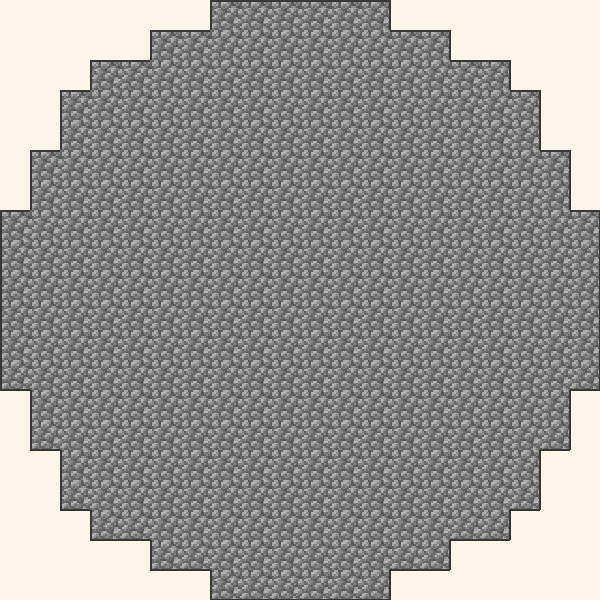
\includegraphics[width=\linewidth]{fig04_2d_d20_euclidean.png}
  \caption{\emph{填充}}
\end{subfigure}\hfill
\begin{subfigure}[t]{0.31\linewidth}\centering
  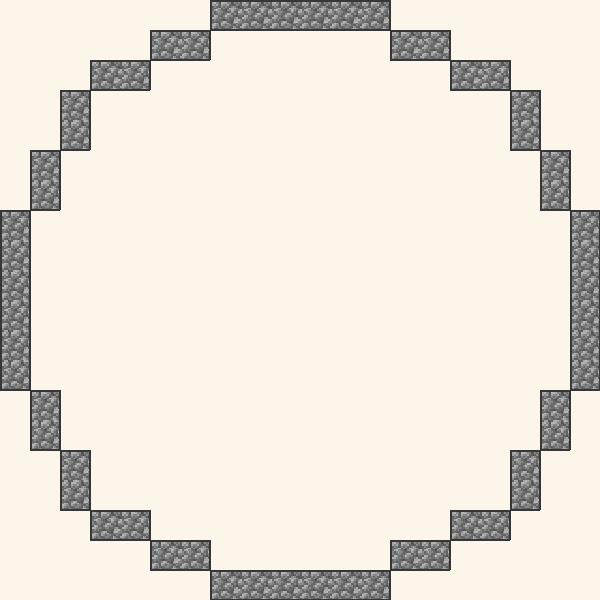
\includegraphics[width=\linewidth]{fig08_2d_d20_thin.png}
  \caption{\emph{薄壳}（一格厚轮廓）}
\end{subfigure}\hfill
\begin{subfigure}[t]{0.31\linewidth}\centering
  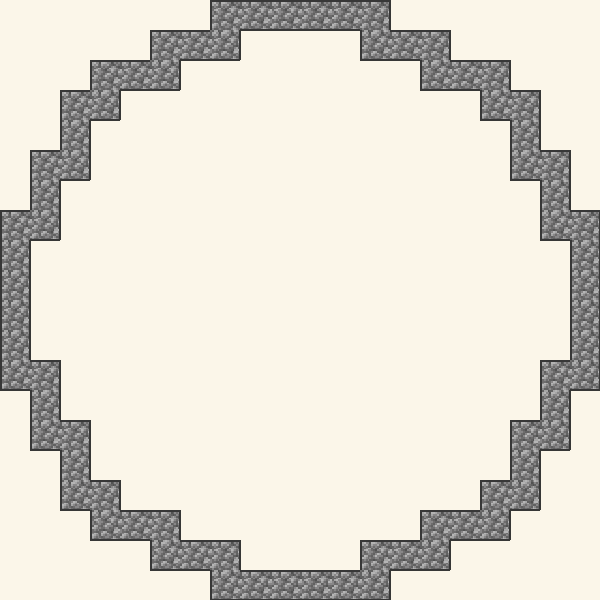
\includegraphics[width=\linewidth]{fig09_2d_d20_thick.png}
  \caption{\emph{厚壳}（带对角桥接）}
\end{subfigure}
\caption{同一直径20欧几里得圆的三种渲染模式。\emph{薄壳}模式对应离散拓扑边界；\emph{厚壳}模式在对角方向添加方块以避免 45 度方向漏洞——这正是水下玻璃穹顶面临的问题：一个对角缝隙就会让水灌进来。}
\label{fig:render-modes}
\end{figure}

\subsection{方块贴图：Block Round 的核心差异}

虽然"哪些体素被选中"的数学独立于贴图，Block Round 还是把每个体素用其在我的世界中的六面标准贴图渲染出来。同一个直径10的球，因方块选择不同而呈现\emph{完全不同}的视觉性格（图\ref{fig:textures}），\emph{而底层算法毫无改变}。这是本教学的核心要点：\emph{形是数学的产物，貌是事后的美学决定}。

\begin{figure}[!htbp]
\centering
\begin{subfigure}[t]{0.31\linewidth}\centering
  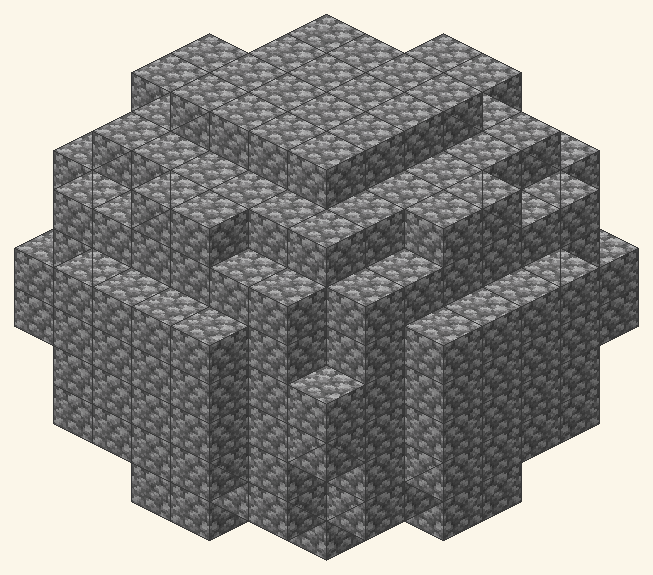
\includegraphics[width=\linewidth]{fig15_3d_sphere_cobblestone.png}
  \caption{\emph{Cobblestone（圆石）}}
\end{subfigure}\hfill
\begin{subfigure}[t]{0.31\linewidth}\centering
  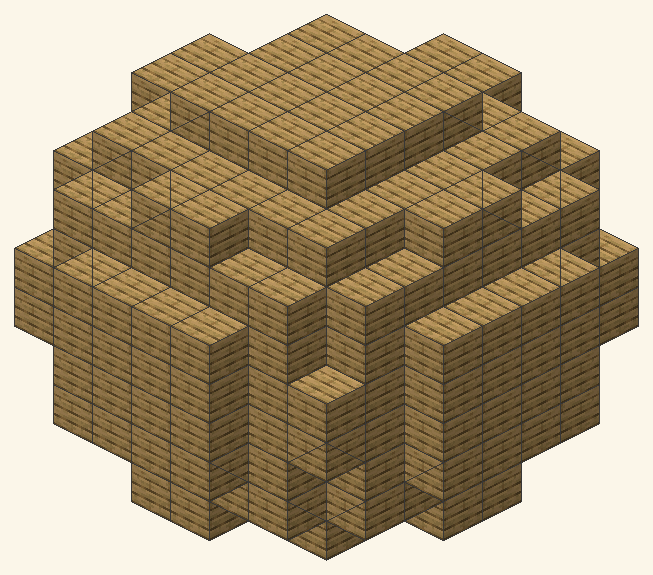
\includegraphics[width=\linewidth]{fig17_3d_sphere_oak.png}
  \caption{\emph{Oak Planks（橡木板）}}
\end{subfigure}\hfill
\begin{subfigure}[t]{0.31\linewidth}\centering
  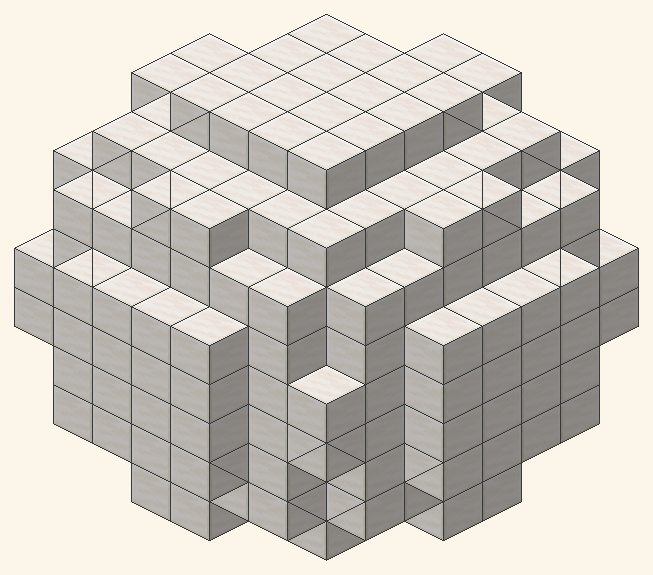
\includegraphics[width=\linewidth]{fig19_3d_sphere_quartz.png}
  \caption{\emph{Quartz Block（石英块）}}
\end{subfigure}
\caption{同一直径10球的三种我的世界贴图。三幅图的体素轮廓\emph{完全相同}——数学没有变化。变化的是视觉性格：\emph{圆石}令人想起中世纪城墙；\emph{橡木板}让人联想到木屋或船舱内部；\emph{石英块}则有现代庙宇的气质。}
\label{fig:textures}
\end{figure}

% =============================================================================
\section{先备知识}\label{sec:prerrequisitos}

本教学序列假设学生已经具备以下基础：

\begin{itemize}[leftmargin=1.3em,itemsep=0.15em,topsep=0.3em]
  \item 平面直角坐标系：定位 $(x, y)$ 与 $(x, y, z)$。
  \item 圆的标准方程（高一必修课）。
  \item 多边形与圆的面积；立方体、棱柱与圆柱的体积（高二必修课）。
  \item 函数的概念：定义域、值域、图像。
  \item 比例与百分比。
  \item 带商带余的整数除法（初中内容）。
\end{itemize}

\emph{可选先备知识（非强制，但有帮助）：}我的世界使用经验。本序列专门考虑了\emph{完全没玩过}我的世界的学生（在网络受限的乡村或山区中学可能出现），可以完全跟上——所有操作都在 Block Round 中进行，浏览器自包含。

如果班级在上述某项必修内容上有明显短板（疫情后这是常见现象，根据 PISA 2022 北京-上海-江苏-浙江数据，城市学生数学成绩仍居全球前列，但学生间差异明显增大），\emph{第~1~课}保留了10分钟的\emph{诊断性诊断}环节，参见 §\ref{aula1}。

% =============================================================================
\section{教学资源}\label{sec:recursos}

\subsection{数字资源}
\begin{itemize}[leftmargin=1.3em,itemsep=0.15em,topsep=0.3em]
  \item Block Round（每生一台\emph{或}每双人一台）；
  \item 多媒体投影仪、HDMI 接口的智能电视或交互式电子白板；
  \item 学校\emph{信息技术机房}\emph{或}学生自带设备（BYOD —— 自带智能手机/平板）；
  \item （选用，第~\ref{aula5}~课）\emph{我的世界 Java 版}或\emph{网易我的世界国服}（含 Litematica 或 Schematica 模组）；亦可使用原版命令 \cmd{/fill} 与 \cmd{/clone}。
\end{itemize}

\subsection{纸质资源}
\begin{itemize}[leftmargin=1.3em,itemsep=0.15em,topsep=0.3em]
  \item 1\,cm 坐标纸，每生两张；
  \item 铅笔、橡皮、30\,cm 直尺；
  \item 彩色铅笔或马克笔（建议以草地绿 \texttt{\#5B8E3F} 与泥土棕 \texttt{\#825432} 为主，对齐 Block Round 配色）；
  \item 练习题册（附录~\ref{ap:exerc}）；
  \item 普通黑板或白板。
\end{itemize}

\subsection{统编教材衔接}\label{sec:pnld}

Block Round \emph{补充}而非\emph{替代}由教育部审定的统编教材。与本序列内容紧密相关的章节：

\begin{itemize}[leftmargin=1.3em,itemsep=0.1em,topsep=0.2em,nosep]
  \item 人教版\emph{普通高中教科书 数学}必修第二册"圆与方程"章；
  \item 人教版\emph{普通高中教科书 数学}选择性必修第一册"圆锥曲线"章；
  \item 人教 A 版必修第二册"立体几何"章节中关于球体积与表面积的部分；
  \item 北师大版、苏教版、湘教版的对应章节；
  \item 上海科技出版社（沪教版）"解析几何"章节（适用于沪、苏自主命题地区）。
\end{itemize}

特别地，统编教材中关于\emph{铺砖问题}、\emph{覆盖与计数}、\emph{格点问题}的内容（高考考点）与 Block Round 的核心问题在数学本质上是等价的，只是术语略有不同。

\subsection{Block Round 的获取方式}

按推荐顺序：

\begin{enumerate}[leftmargin=1.5em,itemsep=0.15em,topsep=0.3em]
  \item \textbf{教师在 GitHub Pages 或校内服务器托管}：通过黑板投影 QR 二维码分发 URL。公开版本：\url{https://vinisouza128.github.io/block-round/}。
  \item \textbf{本地副本}：将项目文件夹拷贝至机房电脑，通过 \emph{file://} 协议打开。
  \item \textbf{智能手机离线}（PWA）：用浏览器联网打开一次后，浏览器即可将其安装为离线应用。
\end{enumerate}

% =============================================================================
\section{适配中国高中教育的多样性}\label{sec:adapt}

中国大陆高中教育在地域、城乡、民族、办学性质等维度都存在显著差异。本序列设计成可在以下各种场景中适用，每种场景对应不同的实施方案。

\subsection{一线/二线城市重点中学（设施完善）}
典型场景：北京四中、人大附中、北师大实验中学、上海中学、华师大二附中、深圳实验、广州执信、南京外国语学校、杭州第二中学、华南师大附中。一般配备完整的信息技术机房、交互式电子白板与稳定的校园 Wi-Fi。许多学校已购置\emph{Minecraft Education Edition} 教育版授权——第~\ref{aula5}~课可完整在此环境中开展。\emph{这是实施本序列最直接的场景。}

\subsection{三四线/地级市省级示范高中}
覆盖全国大部分地级市，例如苏州中学、温州中学、汕头金山中学、银川一中、兰州一中、贵阳一中、昆明一中、玉林高中等。机房设备多数可用但相对老旧。建议采用\emph{BYOD 模式}：以学生自带智能手机为主，双人一组（每组一部手机）。Block Round 在 2018 年以来的 Android 手机上可流畅运行。若我的世界国服访问受限，第~\ref{aula5}~课可改为"假设命令"形式（纸上规划 + 描述效果），不影响概念学习。这是\acc{最常见}的场景。

\subsection{中等职业学校 / 国际部 / 科技特色高中}
中等职业学校（"中职"）、技师学院，以及科技特色高中（如学军中学、中科大附中、清华附中、北大附中数学班）。这类学校通常有较强的实验设施与编程教学传统。建议把\emph{第~\ref{aula2}~课的 Bresenham 算法}扩展为 Python 实现（信息技术课时配合）；并把\emph{第~\ref{aula5}~课}延展为完整的服务器部署项目（学生可负责服务器搭建与运维）。与\emph{游戏开发}相关的中职专业（游戏美术、游戏程序）尤其能从中获益。国际部（IB/AP/A-Level 课程）可作为 IB 数学 Internal Assessment（IA）或 AP Computer Science Principles 项目的主题。

\subsection{县乡级乡镇普通高中（基础设施有限）}
广大县级与乡镇普通中学，覆盖中西部、东北、西南山区。机房设备有限，但学生对\emph{几何应用}有较强的直观经验（梯田、村镇规划、传统民居建造）。建议使用纯纸质版本（附录~\ref{ap:adapt-analog}）或单一教师演示设备。第~\ref{aula3}~课可结合当地的圆形农场、谷仓、晒谷场等传统建筑实例，把\emph{具身的几何}与\emph{符号化的几何}对接。

\subsection{民族学校（少数民族中学，双语教学）}
依据《民族区域自治法》设立的民族类中学使用本民族语言与普通话双语教学。蒙古族、藏族、维吾尔族、朝鲜族、回族、壮族、苗族、彝族等55个少数民族都有对应的民族中学（民族班、民族部）。本序列可\emph{借助本民族建筑与纹样资源得到丰富}：蒙古包的同心圆几何（内蒙古、新疆）、藏族碉房与曼陀罗几何（西藏、四川甘孜）、傣族竹楼的高架几何（云南西双版纳）、苗族吊脚楼的斜坡梯田几何（贵州、湖南）、维吾尔族民居的拱门几何（新疆喀什）、客家土楼的圆形几何（福建永定、南靖）。\emph{由民族语文教师与本地老一辈手艺人（毡匠、木匠、铁匠）共同参与是关键。}第~\ref{aula3}~课的 \emph{活动~\ref{at:34}} 是这一方向的入口。

\subsection{西部边远地区高中（"组团式援疆援藏"项目支持的中学）}
新疆、西藏、青海、甘肃、宁夏、贵州、云南等边远省份的县级与地区中学。这类学校得益于\emph{教育部直属师范大学公费师范生}、\emph{组团式援疆援藏}、\emph{东西部协作}等国家支援计划。教学条件波动较大。Block Round 的 PWA 离线特性在低带宽地区尤具价值。推荐使用单台教师设备演示 + 纸质学生作业的混合模式，并优先选择附录~\ref{ap:adapt-analog}~的纸质活动。

\subsection{成人高中 / 国家开放大学（成人继续教育）}
成人高中、业余高中、函授教育、远程教育、电视大学、国家开放大学的成人学习者。Block Round 的友好界面与游戏化主题对成人学习者也很有效（很多70后、80后家长本身是早期我的世界玩家或通过子女接触此游戏）。建议每个活动的时间缩减约 20\%（成人课时通常较短），并优先口头讨论而非长篇书面作业。第~\ref{aula5}~课可改为\emph{选学}，重点放在第~1--4~课。

\subsection{100 分钟"大课"合并模式}
适用于实行"大课"或长时段教学的实验高中：第 1+2 课合并为一节 100 分钟课，第 3+4 课合并为一节，第 5 课单独 50 分钟（或合并 100 分钟以延长建造时间）。共 3 节 100 分钟 + 1 节 50 分钟，或 2 节 100 分钟 + 1 节 200 分钟（最后一节用于完整建造）。

\subsection{各省（直辖市）高考与新课标对接}

新高考改革自2014年起逐步推行，至2024年已覆盖29个省份的"3+1+2"或"3+3"模式。各省教育考试院在课标基础上对数学高考做了不同程度的本地化要求：

\begin{center}
\small
\begin{tabularx}{\textwidth}{@{}p{0.16\textwidth}p{0.22\textwidth}X@{}}
\toprule
\textbf{省/直辖市} & \textbf{高考模式} & \textbf{圆与圆锥曲线、立体几何的命题特点} \\
\midrule
北京 & 自主命题，"3+3" 模式 & 圆与圆锥曲线常作为压轴大题；立体几何强调空间向量方法；新高考改革标杆。 \\
\addlinespace[3pt]
上海 & 自主命题，"3+3" 模式 & 平面解析几何 + 立体几何并重；圆锥曲线题型设计精巧，重视分类讨论。 \\
\addlinespace[3pt]
江苏 & 新高考"3+1+2"（2021年起，此前自主命题2008--2020） & 解析几何传统强项；圆与椭圆压轴题极具挑战性；新高考后向全国卷靠拢。 \\
\addlinespace[3pt]
浙江 & 新高考"3+3"，选考7选3 & 圆锥曲线与立体几何均有压轴题分布；强调建模与综合应用。 \\
\addlinespace[3pt]
广东 & 新高考"3+1+2"，全国卷 & 圆的方程为必考；立体几何大题强调坐标法；选考结构灵活。 \\
\addlinespace[3pt]
山东 & 新高考"3+3" & 圆锥曲线综合大题；立体几何与空间向量；近年改革步伐较快。 \\
\addlinespace[3pt]
四川/重庆/西部 & 全国卷 & 圆与直线必考；立体几何常作为大题；解析几何压轴较为传统。 \\
\bottomrule
\end{tabularx}
\end{center}

\subsection{线上/混合式教学}
Block Round 的网页性质使其天然兼容线上教学。教师在\emph{钉钉课堂}、\emph{腾讯课堂}、\emph{ClassIn}、\emph{智学网}或地方教育云平台（如北京"空中课堂"、上海"空中课堂"、广东"粤教翔云"）共享屏幕；学生在自己的设备上同步操作。坐标纸活动可拍照后由家长上传至\emph{微信}群、\emph{钉钉}班级群或学校 LMS。第~\ref{aula5}~课可在班级共享的我的世界服务器（国服或自建私服）中进行，全班学生在虚拟世界中协同建造。教育部"国家中小学智慧教育平台"亦支持本序列的发布与分享。

% =============================================================================
\section{教学序列}\label{sec:sequencia}

教学序列遵循\acc{激发动机 --- 提出问题 --- 系统化 --- 综合应用}的结构，参考了"三段式教学"以及强调"从学生已有经验出发"的本土教学传统。每节 50 分钟的课遵循高中生的认知节奏，将不超过 15 分钟的讲授环节与实践活动交替进行。

% =============================================================================
\subsection{第~1~课 ——"游戏是怎么用方块画球的？"}\label{aula1}

\subsubsection*{本课目标}
建立\emph{离散光栅化}这一核心问题，并把它确立为一个\emph{真正的数学问题}；调动圆的方程；介绍 Block Round。让学生认识到：本课的核心问题——\emph{怎样决定哪些方块该上色？}——正是每个我的世界玩家在游戏里建一个球时面临的真实问题。

\begin{huodong}[1.1 —— 激发动机 \quad\tempo{10 分钟}]
\textbf{策略：}\emph{think--pair--share}（独立思考 -- 同伴讨论 -- 全班分享）。\\[0.4em]
\textbf{步骤：}
\begin{enumerate}[leftmargin=1.5em,itemsep=0.2em,topsep=0.3em,nosep]
  \item 投影（或在黑板上画）三个我的世界中的经典建筑：以石头（Stone）为基础的玻璃穹顶（B站上任何一位 UP 主的圆球教程截图）；网易我的世界国服热门服务器上集体建造的"巨大球体"（可来自抽风Crazy\_、籽岷ZeMin、Joe粥等知名 UP 主的视频）；以及在我的世界中复刻的中国文化形象（春晚吉祥物、孙悟空、京剧脸谱、电竞选手头像、网红 IP）。
  \item 向全班提问：\emph{"仔细看。游戏是怎么决定该把哪些方块放在哪里来构成一个球的？是不是游戏里有一只'神奇的圆规'？"}
  \item 每位学生独立写下自己的回答（1 分钟），然后与同桌讨论（2 分钟）。
  \item 集体收集：将关键回答记录在黑板侧边。引导学生意识到根本观察：\emph{"游戏只能放完整的方块——它怎么决定放哪些？"}
\end{enumerate}
\end{huodong}

\begin{huodong}[1.2 —— 提出问题 \quad\tempo{15 分钟}]
\textbf{策略：}手工绘制 vs. 形式定义的对照。\\[0.4em]
\textbf{材料：}坐标纸、铅笔。\\[0.4em]
\textbf{步骤：}
\begin{enumerate}[leftmargin=1.5em,itemsep=0.2em,topsep=0.3em,nosep]
  \item 每位学生拿到半张坐标纸，标记一个 $11 \times 11$ 方格区域的中心点。
  \item 指令：\emph{"画出你认为最好的、直径10（半径5）的圆。\emph{把每个小方格想象成我的世界里的一个圆石方块。}你们有 4 分钟。"}
  \item 时间到后，三到四位学生上黑板，在用粉笔/记号笔画好的方格里复现自己的方案。
  \item 教师引导观察：\emph{"看好。你们画的是同一个图吗？为什么不是？谁对了？如果你们每个人都在同一个班级共享的我的世界服务器上建这个球，会出什么问题？"}
  \item 系统化：没有\emph{唯一}答案（图\ref{fig:comp-d10} 已在 §\ref{sec:justificativa} 中印证）。每位学生隐含地采用了不同的\acc{判据}来决定方格的归属。
\end{enumerate}

\textbf{民族数学札记：}借此契机指出：\emph{这种"多种答案都对"的现象正是民族数学（ethnomathematics）研究的对象}（乌比拉坦·杜安布罗西奥，已被译介进入中国；张维忠《文化传统与数学教育现代化》，北京师范大学）。不同文化以不同方式做"同一道题"。\emph{中国的我的世界玩家社群本身就是一种文化群体，有自己的"民族数学"}，通过 B站中文教程、网易我的世界国服服务器、微信公众号、QQ 群口耳相传。
\end{huodong}

\begin{huodong}[1.3 —— 系统化 \quad\tempo{15 分钟}]
\textbf{策略：}以板书为支撑的对话式讲解。\\[0.4em]
\textbf{内容：}

以原点为中心、半径为 $r$ 的圆的隐式方程为：

\begin{gongshi}
\centering
$\displaystyle x^2 + y^2 \;=\; r^2$
\end{gongshi}

圆\emph{内部}的点满足 $x^2 + y^2 < r^2$；\emph{外部}的点满足 $x^2 + y^2 > r^2$。该方程推广到半轴为 $r_x, r_y$ 的椭圆：

\begin{gongshi}
\centering
$\displaystyle \left(\dfrac{x}{r_x}\right)^{\!2} + \left(\dfrac{y}{r_y}\right)^{\!2} \;=\; 1$
\end{gongshi}

在方块（体素）网格上，挑战是决定哪些\acc{方格}应当被纳入"内部"。不同的判定准则会产生不同的结果。Block Round 实现了\emph{三种}判据：

\begin{itemize}[leftmargin=1.3em,itemsep=0.15em,topsep=0.3em]
  \item \acc{欧几里得判据}：方格的中心点 $(i + \tfrac{1}{2},\, j + \tfrac{1}{2})$ 是否在圆内？
  \item \acc{Bresenham 算法}：1965 年发表的经典算法，只使用整数运算。
  \item \acc{阈值判据}：方格的某个\emph{角点}是否在圆内？
\end{itemize}

\textbf{现场演示：}教师打开 Block Round，将直径设为 10，依次切换三个算法，让学生观察差异。强调：三幅图都\emph{在不同判据下数学正确}。再演示更换贴图——圆变成 cobblestone、oak\_planks、diamond、glowstone——而\emph{形状不变}。\emph{这是 Block Round 的核心点：形是数学，貌是事后审美。}
\end{huodong}

\begin{huodong}[1.4 —— 综合应用 \quad\tempo{10 分钟}]
\textbf{策略：}个人即时应用。\\[0.4em]
\textbf{指令：}\emph{"回到坐标纸。\acc{严格}地按欧几里得判据重新画直径 10 的圆：当且仅当方格的中心点 $(i + 0.5,\, j + 0.5)$ 到圆心的距离不超过 5 时，把它涂黑。"}

完成后，将自己的图与 Block Round 在欧几里得算法下、直径 10 的输出对比——参考图\ref{fig:comp-d10}~(a)。\emph{两者应当一致。}
\end{huodong}

\begin{minecraft}[与游戏的衔接]
在\emph{我的世界 Java 版}安装了 WorldEdit 模组后，命令 \cmd{//sphere stone 5} 画出的图形与 Block Round 在 \emph{Bresenham} 算法、直径10 下的输出完全相同。在国服里游玩的学生可以在家里验证——建造结果一致。\emph{这意味着：我们在课堂上学的不是游戏的简化模拟，而是游戏背后用的同一套数学。}
\end{minecraft}

\subsubsection*{家庭作业（选做）}
用直径 8 和 14 重复活动 1.4。下节课带上三张图。会玩我的世界的同学：尝试在游戏中直接复现——用 \cmd{/setblock} 一块一块放，或者用 \cmd{//sphere}（如果有 WorldEdit），然后拍照存档。

% =============================================================================
\subsection{第~2~课 ——"三个算法，三幅图，三套建造方案"}\label{aula2}

\subsubsection*{本课目标}
深入理解三个算法是\emph{不同的数学定义}，并定量比较结果；包括把"我建这个球要采集多少方块"这件事纳入对比——一个生存模式建造者关心的实际问题。

\begin{huodong}[2.1 —— 回顾 \quad\tempo{5 分钟}]
快速收回家庭作业中的图，观察班内的多样性，宣布本课目标：\emph{"今天我们要用'放大镜'看三个算法，并发现：为什么 Bresenham 被誉为计算机科学的'明珠'——而中国的我的世界玩家虽然没听过这个名字，却每天都在用它。"}
\end{huodong}

\begin{huodong}[2.2 —— 欧几里得算法 \quad\tempo{10 分钟}]
形式化。对方格 $(i, j)$，计算标准化坐标：

\begin{gongshi}
\centering
$\displaystyle d_x = \dfrac{i + \tfrac{1}{2} - c_x}{r_x},\qquad d_y = \dfrac{j + \tfrac{1}{2} - c_y}{r_y}$
\end{gongshi}

方格被纳入当且仅当 $d_x^{\,2} + d_y^{\,2} \leq 1$。

\textbf{板书：}显式求解 $c_x = c_y = 5$、$r_x = r_y = 5$、方格 $(2, 1)$ 的情形。此时 $d_x = (2.5 - 5)/5 = -0.5$，$d_y = (1.5 - 5)/5 = -0.7$，因此 $d_x^2 + d_y^2 = 0.25 + 0.49 = 0.74 \leq 1$。方格\emph{属于内部}。\\

请学生计算方格 $(0, 0)$（结果如何？）。讨论。
\end{huodong}

\begin{huodong}[2.3 —— Bresenham 算法 \quad\tempo{15 分钟}]\label{at:23}
\textbf{历史背景：}Jack Bresenham 于 1965 年在 IBM 工作期间发表了该算法。在他之前，画一条直线需要浮点运算——在那个年代的计算机上代价昂贵。Bresenham 证明可以\emph{只用整数}——加法与比较——就能画出来。后来由 Pitteway（1967, IBM）等人推广到椭圆。

对圆的版本使用一个\emph{决策参数} $d$。从 $(x{=}0,\, y{=}R)$ 出发，$d_0 = 1 - R$。在 $0$--$45^\circ$ 八分之一象限的每一步：

\begin{gongshi}
\centering
$\begin{cases}
\text{若 } d < 0: & \text{下一步: } (x{+}1,\, y),\; d \mathrel{+}= 2x+3 \\
\text{若 } d \geq 0: & \text{下一步: } (x{+}1,\, y{-}1),\; d \mathrel{+}= 2(x-y)+5
\end{cases}$
\end{gongshi}

\textbf{板书演示：}对 $R = 5$ 一步步执行算法，每次迭代记录 $x, y, d$。八个象限通过对称获得。\\

\textbf{与我的世界的衔接：}\emph{WorldEdit} 模组（Sponge、Bukkit、Paper、Fabric 都有版本）的 \cmd{//sphere} 命令实现了 Bresenham 3D 的变体——同一套 1965 年的数学，今天运行在全球数百万台我的世界服务器上。\emph{你现在学的正是游戏在你输入} \texttt{//sphere stone 8} \emph{时偷偷做的事。}

\textbf{与信息学奥赛的衔接：}Bresenham 算法是\href{https://www.noi.cn/}{全国青少年信息学奥林匹克竞赛（NOIP/NOI）}的经典题源，且在国际信息学奥林匹克（IOI）中国队的训练教材中常被提及。中国信息学奥赛由中国计算机学会（CCF）组织，对希望走"信息学保送/强基"路径的学生是关键。

\textbf{教学说明：}如果班级对决策参数 $d$ 的代数推导有困难，可仅作为\emph{规则}给出（不证明决策函数的来源）。完整论证在技术文档 \texttt{Block\_Round\_Math\_zh-CN.pdf} §5 中。
\end{huodong}

\begin{huodong}[2.4 —— 阈值算法 \quad\tempo{10 分钟}]
对每个方格 $(i, j)$，找到距圆心\emph{最近的角点}：

\begin{gongshi}
\centering
$\displaystyle n_x = \mathrm{clamp}(c_x,\, i,\, i{+}1),\qquad n_y = \mathrm{clamp}(c_y,\, j,\, j{+}1)$
\end{gongshi}

方格被纳入当且仅当 $\left(\dfrac{n_x - c_x}{r_x}\right)^{\!2} + \left(\dfrac{n_y - c_y}{r_y}\right)^{\!2} \leq 0.94$。

\textbf{为什么是 $0.94$ 而不是 $1$？}经验上，取 $1$ 会在四个基本方向上出现一格的"尖刺"。略低于 $1$ 的阈值消除这种伪影。\emph{这是基于视觉检验的工程决定}——一个重要的例子：纯粹的理论数学有时并不够。借用我们前面的话：\enquote{最终发言权}不在公式，而在理论与实践的对话之中。

\textbf{何时在我的世界里用阈值：}对于\emph{远观}的穹顶或半球建筑（山顶神庙、岛上陵墓、海面浮城），阈值算法产生的轮廓略\enquote{饱满}一些，在迷雾与环境光遮蔽下视觉读取更佳。代价是约 5--10\% 更多方块。建议用于"远观美感优先于材料经济"的项目。
\end{huodong}

\begin{huodong}[2.5 —— 定量比较 \quad\tempo{10 分钟}]\label{at:25}
\textbf{双人小组实践。}在 Block Round 中（或教师中央演示）：
\begin{enumerate}[leftmargin=1.5em,itemsep=0.15em,topsep=0.3em,nosep]
  \item 设定直径 20、\emph{填充}模式（图\ref{fig:comp-d20} 展示了三个算法的预期结果）。
  \item 启用画布角落的 \emph{Info chip}（信息提示）。记录三个算法各自的面积。
  \item 计算连续面积：$\pi r^2 = \pi \cdot 10^2 \approx 314.16$。
  \item 对每个算法，计算相对误差：$\dfrac{|\text{离散面积} - \text{连续面积}|}{\text{连续面积}} \times 100\%$。
  \item 按与连续值的接近程度排序三个算法。
  \item \emph{与我的世界的衔接：}\emph{"如果你们在生存模式下要造这三个球，哪个最少要跑仓库取圆石？哪个最多？"}最少（欧几里得）与最多（阈值）之间的 stack 差可达整整 1 stack（64 块）。
\end{enumerate}

\textbf{预期结果：}欧几里得通常误差最小（低于 $2\%$）；阈值会略微高估；Bresenham 居中。集体确认。
\end{huodong}

\begin{figure}[!htbp]
\centering
\begin{subfigure}[t]{0.31\linewidth}\centering
  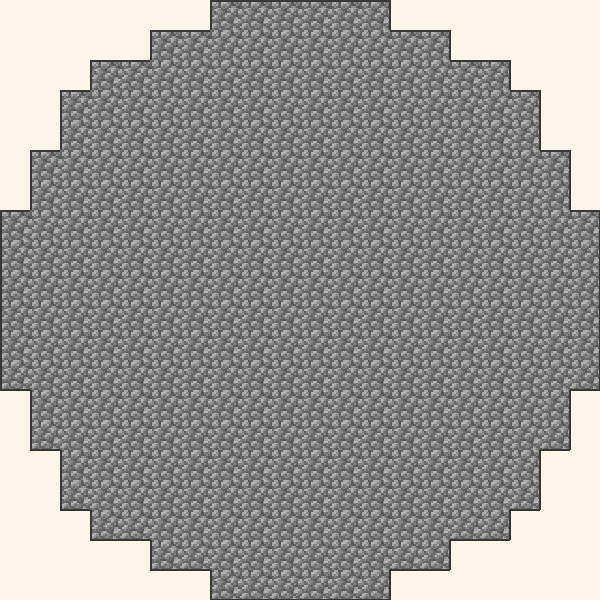
\includegraphics[width=\linewidth]{fig04_2d_d20_euclidean.png}
  \caption{\emph{欧几里得}}
\end{subfigure}\hfill
\begin{subfigure}[t]{0.31\linewidth}\centering
  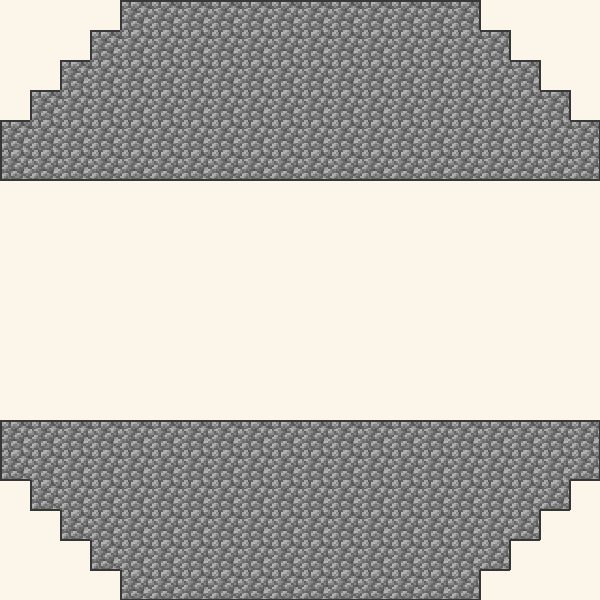
\includegraphics[width=\linewidth]{fig05_2d_d20_bresenham.png}
  \caption{\emph{Bresenham}}
\end{subfigure}\hfill
\begin{subfigure}[t]{0.31\linewidth}\centering
  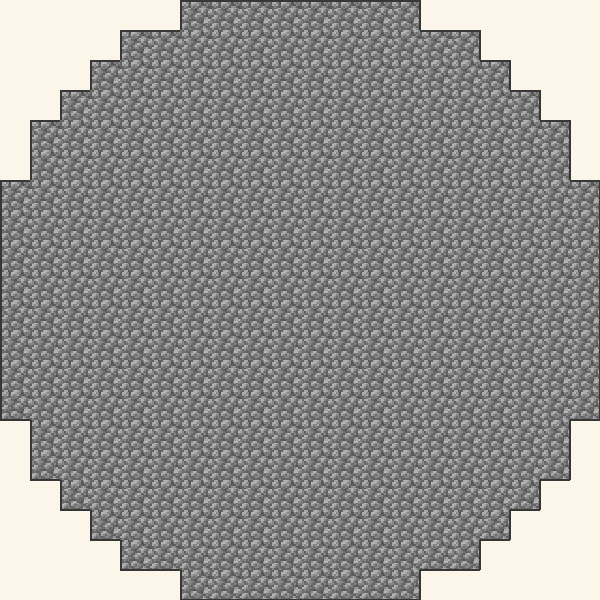
\includegraphics[width=\linewidth]{fig06_2d_d20_threshold.png}
  \caption{\emph{阈值}}
\end{subfigure}
\caption{同一直径 20 圆在三个算法下的结果，使用圆石贴图。直径增大后，差异更细微——肉眼看上去三幅图相似。可借此提醒学生：在更小的直径下（图\ref{fig:comp-d10}）差异更显著。}
\label{fig:comp-d20}
\end{figure}

\begin{minecraft}[方块计数：Block Round vs WorldEdit]
课后试试（如果有我的世界 + WorldEdit）：在服务器执行 \cmd{//sphere stone 10}，数一下方块数。与 Block Round 在 Bresenham 算法、$D = 20$ 下 \emph{Info chip} 显示的方块数对比。两者应一致（\emph{或}相差 0--4 块——实现细节差异）。如果你发现有一致的偏差，那就是一个\emph{真实的数学发现}。
\end{minecraft}

% =============================================================================
\subsection{第~3~课 ——"从椭圆到椭球：进入第三维"}\label{aula3}

\subsubsection*{本课目标}
把椭圆方程推广到椭球；引入体素、离散体积与平面切割。建立与中华视觉文化遗产以及网易我的世界国服著名建造作品的桥梁。

\begin{huodong}[3.1 —— 从 2D 方程到 3D \quad\tempo{15 分钟}]\label{at:31}
在平面直角坐标系上加上第三个坐标 $z$。椭圆的隐式方程自然推广：

\begin{gongshi}
\centering
$\displaystyle \left(\dfrac{x}{r_x}\right)^{\!2} + \left(\dfrac{y}{r_y}\right)^{\!2} + \left(\dfrac{z}{r_z}\right)^{\!2} \;=\; 1$
\end{gongshi}

当 $r_x = r_y = r_z = r$ 时，恢复为\acc{球}： $x^2 + y^2 + z^2 = r^2$（图\ref{fig:3d-shapes}）。

\textbf{体素：}3D 网格中的一个方格被称为\emph{体素}（voxel，\emph{volume element}）。在我的世界中，每个体素就是一块 $1 \times 1 \times 1$ 的方块。属于判据与 2D 情形完全相同，只是加上一个 $z$ 坐标：

\begin{gongshi}
\centering
$\displaystyle a_x^2 + a_y^2 + a_z^2 \leq 1,\quad \text{其中 } a_\xi = \dfrac{\xi + \tfrac{1}{2} - c_\xi}{r_\xi}$
\end{gongshi}

\textbf{现场演示：}打开 Block Round 的 3D 模式，在 \emph{Sphere} 与 \emph{Ellipsoid} 之间切换，用鼠标拖动旋转视角，观察体素结构。
\end{huodong}

\begin{figure}[!htbp]
\centering
\begin{subfigure}[t]{0.45\linewidth}\centering
  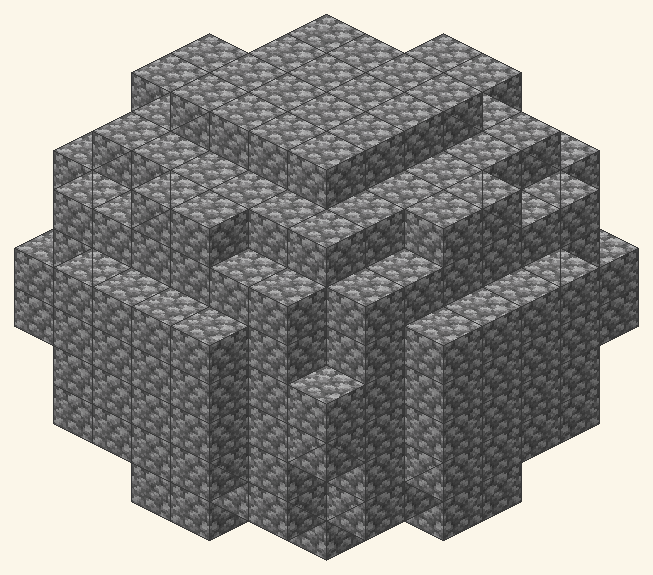
\includegraphics[width=\linewidth]{fig10_3d_sphere_d12.png}
  \caption{直径10的球（$r_x = r_y = r_z = 5$）。}
\end{subfigure}\hfill
\begin{subfigure}[t]{0.45\linewidth}\centering
  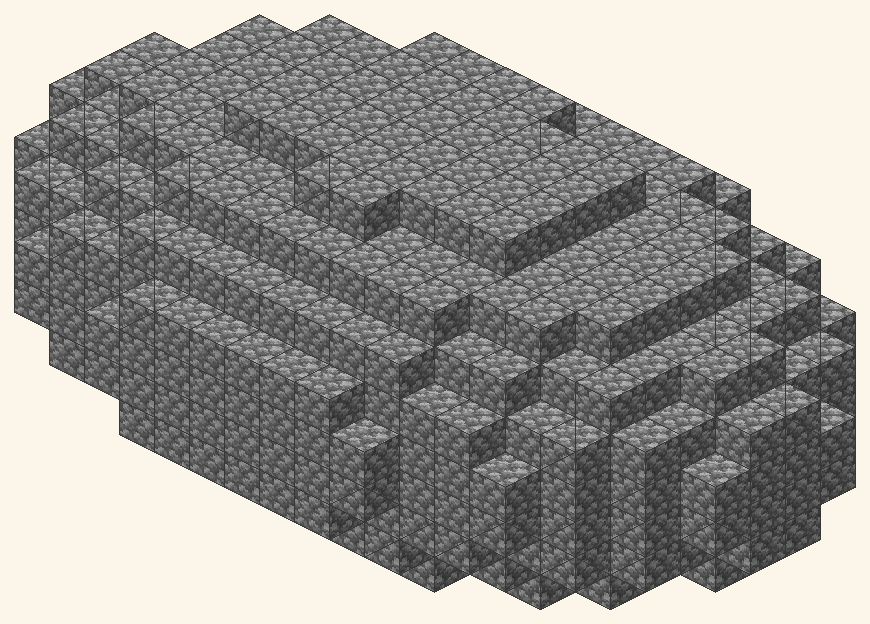
\includegraphics[width=\linewidth]{fig11_3d_ellipsoid.png}
  \caption{椭球 $W = 20, H = 10, D = 12$。}
\end{subfigure}
\caption{3D 体素化。每个小立方体是一个体素（即我的世界的一块方块）；它的中心坐标 $(i, j, k)$ 被代入隐式方程进行判定。可见的"楼梯状"表面是体素化的典型特征——也正是我的世界视觉风格的来源。}
\label{fig:3d-shapes}
\end{figure}

\begin{huodong}[3.2 —— 连续体积 vs 离散体积 \quad\tempo{15 分钟}]\label{at:32}
椭球的连续体积是经典结果：

\begin{gongshi}
\centering
$\displaystyle V \;=\; \dfrac{4}{3}\,\pi\, r_x\, r_y\, r_z$
\end{gongshi}

当 $r_x = r_y = r_z = r$ 时，$V = \tfrac{4}{3}\pi r^3$。这是\acc{高考高频考点}（立体几何，几乎每年全国卷都有），也是\hyperref[sec:obmep]{高中数学联赛}的常见命题方向——尤其是涉及数值近似的题型。

\textbf{双人小组活动：}
\begin{enumerate}[leftmargin=1.5em,itemsep=0.15em,topsep=0.3em,nosep]
  \item 计算直径 12 的球（$r = 6$）的连续体积：$V = \tfrac{4}{3}\pi \cdot 216 \approx 904.78$。
  \item 在 Block Round 中生成 $D = 12$、\emph{填充}模式的球，启用 \emph{Info chip}，记录离散体积（方块数）：约 $V_{\mathrm{disc}} \approx 904$ 块。\emph{相对误差约 $0.1\%$ —— 印象深刻。}
  \item 在同一信息提示上，观察记法 $904 = 14 \times 64 + 8$：游戏告诉一个生存玩家\emph{"你需要 14 整 stack 的圆石 + 1 个有 8 块的 stack"}。
  \item 对 $D = 16$ 重复一次（$V_{\mathrm{cont}} \approx 2\,144$；$V_{\mathrm{disc}} \approx 2\,145$）。注意对偶数 $D$ 可能出现\emph{正}误差（高估，因为中心位于格子间）。
\end{enumerate}

\textbf{说明：}$\text{离散体积}/\text{连续体积} \to 1$ 当 $D \to \infty$。对小 $D$，差异较大——这是数学事实：离散化\emph{确实}改变了体积。
\end{huodong}

\begin{huodong}[3.3 —— 平面切割 \quad\tempo{10 分钟}]\label{at:33}
Block Round 允许沿三个不同方向切割椭球。每次切割是对体素中心坐标的\acc{线性不等式}：

\begin{gongshi}
\centering
$\begin{array}{lcl}
\text{X 轴：} & x \geq \mathit{cut} & \Rightarrow \text{丢弃该体素} \\
\text{Y 轴：} & y \geq \mathit{cut} & \Rightarrow \text{丢弃该体素} \\
\text{对角：} & x + y \geq \mathit{cut} & \Rightarrow \text{丢弃该体素}
\end{array}$
\end{gongshi}

图\ref{fig:cortes} 展示了三种 50\% 切割。

\textbf{引导讨论：}\emph{"为什么对角切的幅度是 $D_x + D_y$ 而不是 $D_x$？斜边在哪里？"}引导学生认识到：在矩形包围盒中，$x + y$ 的取值范围在 $0$ 到 $D_x + D_y$ 之间。\emph{在我的世界中，对一个球进行 Y 轴 50\% 切割就得到经典的"穹顶"——球的上半部分——这就是数以千计的服务器上覆盖庙宇、观测台、竞技场所用的同一种结构。}
\end{huodong}

\begin{figure}[!htbp]
\centering
\begin{subfigure}[t]{0.31\linewidth}\centering
  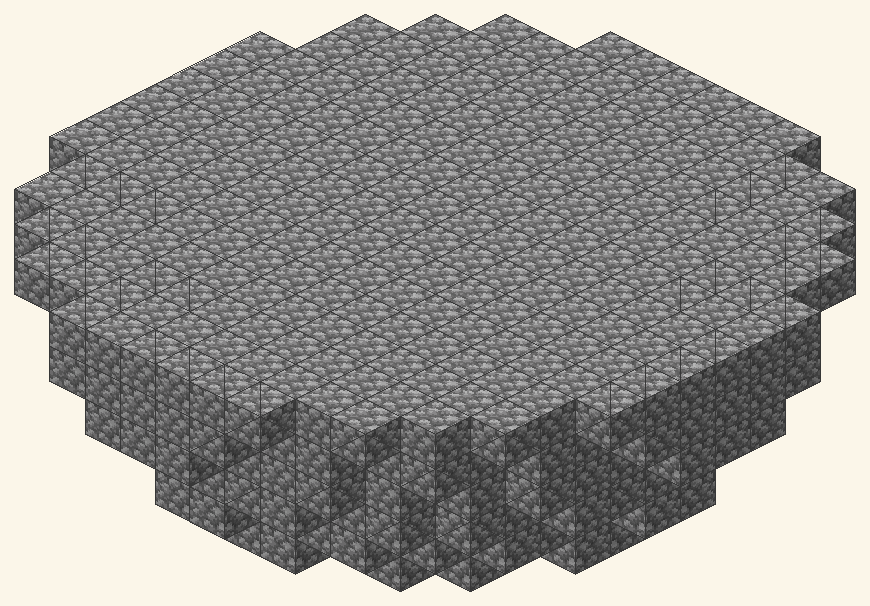
\includegraphics[width=\linewidth]{fig12_3d_cut_y50.png}
  \caption{Y 轴 50\% 切割 —— 经典\emph{穹顶}。}
\end{subfigure}\hfill
\begin{subfigure}[t]{0.31\linewidth}\centering
  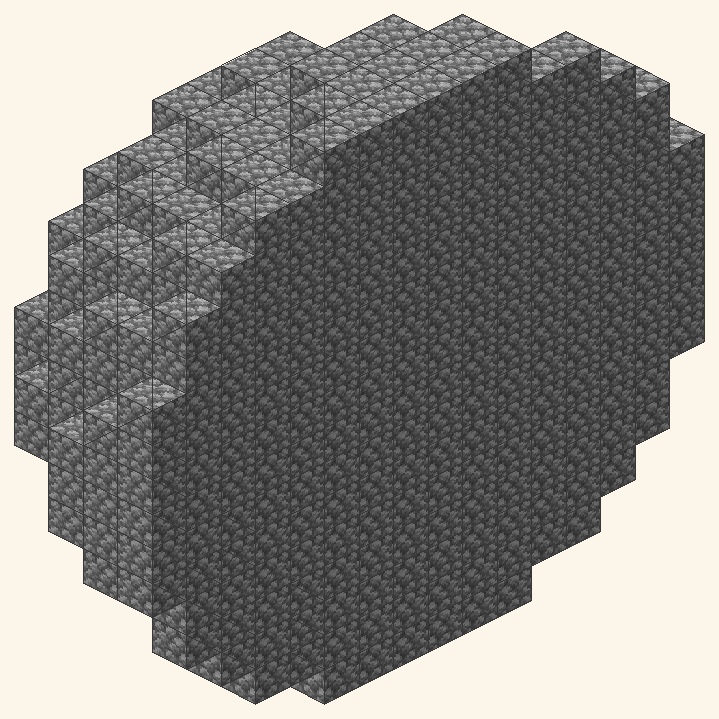
\includegraphics[width=\linewidth]{fig13_3d_cut_x50.png}
  \caption{X 轴 50\% 切割 —— 侧向\emph{半球}。}
\end{subfigure}\hfill
\begin{subfigure}[t]{0.31\linewidth}\centering
  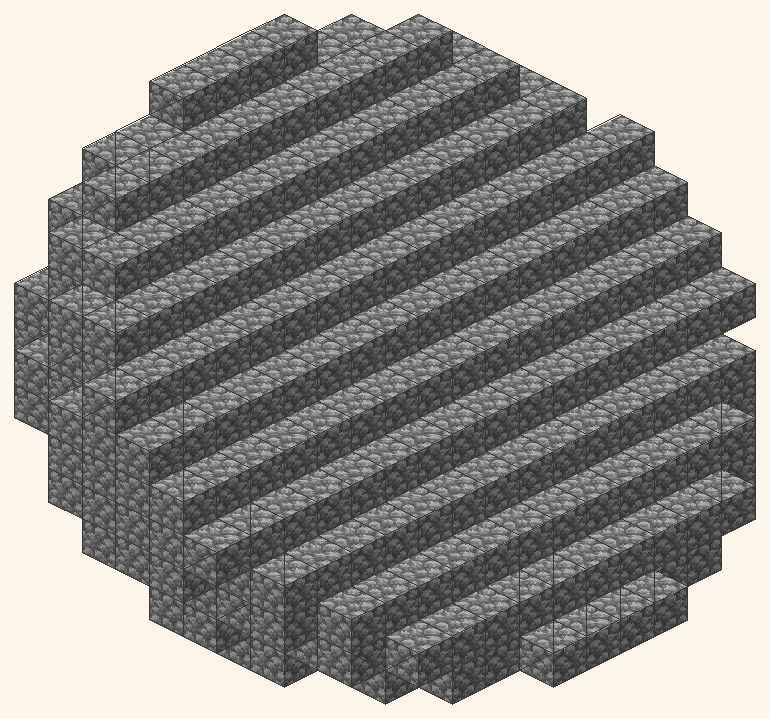
\includegraphics[width=\linewidth]{fig14_3d_cut_diag50.png}
  \caption{对角 50\% 切割 —— 斜置\emph{半碗}。}
\end{subfigure}
\caption{同一直径 16 椭球的三种平面切割，皆保留 50\% 体积。注意对角切割的阶梯纹路：它暴露了连接两轴的斜边。每种切割对应不同的我的世界建造方案：庙宇穹顶、侧向竞技场、喷泉式半圆剧场。}
\label{fig:cortes}
\end{figure}

\begin{huodong}[3.4 —— 与中华视觉文化遗产对话 \quad\tempo{10 分钟}]\label{at:34}
\emph{与语文、艺术、历史的跨学科衔接。本活动落实课标中关于文化认同与遗产传承的要求。}

投影（或印刷分发）五幅图像与素材：

\begin{itemize}[leftmargin=1.3em,itemsep=0.2em,topsep=0.3em,nosep]
  \item \acc{国家大剧院}（Paul Andreu，北京，2007）：一个巨大的钛合金\emph{扁椭球}穹顶——直接对应我们正在研究的椭球；\acc{鸟巢}（国家体育场，2008奥运，Herzog \& de Meuron + 李兴钢 + 艾未未）的钢架交织呈现了体素级别复杂度；\acc{CCTV 大楼}（Rem Koolhaas，北京）的非欧几何造型；\acc{苏州博物馆}（贝聿铭，2006）的几何屋顶与传统园林的几何线条；\acc{北京大兴国际机场}（Zaha Hadid）的星形参数化曲面。这些建筑大师在建筑尺度上实现了我们正在学习的二次曲面。

  \item \acc{故宫太和殿屋顶}的反曲线、\acc{北京天坛祈年殿}（圆形三重檐，直径 30 米）、\acc{客家土楼}（福建永定/南靖的圆形/方形夯土建筑——直接的圆几何与体积计算！）、\acc{布达拉宫}的梯形几何外墙：传统中华建筑通过几百年口耳相传的工匠经验，沉淀了丰富的空间几何知识——\emph{体素化}的隐含智慧，只是没用这个名字。

  \item \acc{良渚文化玉琮}（外方内圆，5300--4300 年前——直接对应"直方圆"几何！UNESCO 世界遗产）、\acc{龙山文化黑陶}（4500--2000 BC）、\acc{殷墟青铜器}（商朝）、\acc{三星堆青铜面具}（古蜀文化）、\acc{兵马俑}（秦代，西安——体素式人物列阵）。这些是中华文明早期的几何与立体造型记录。

  \item \acc{传统几何纹样}：青铜器的饕餮纹、回纹（商周——直接的体素几何！）、\acc{苏州园林漏窗}（千变万化的几何窗格）、\acc{故宫琉璃瓦/方砖排列}（直接的光栅化！）、\acc{景德镇青花瓷}纹样、\acc{苏绣/蜀绣/湘绣/粤绣}的几何图案、\acc{苗族银饰}几何、\acc{藏族唐卡曼陀罗}（mandala，同心圆几何）、\acc{剪纸 jianzhi}（对称性 —— 直接对应 $\mathbb{Z}_2^2$ 群！）。这些是\emph{活生生的}中国本土几何传统，比计算机出现早数千年。

  \item \acc{网易我的世界国服与 B站玩家社群的作品}：在国服服务器（如末日方块、混服等）以及由抽风Crazy\_、籽岷ZeMin、Joe粥、锐刻五Reek\_、小宝Babyfu 等知名 UP 主主持的项目中，可以找到大量穹顶、球体、拱门的建造时序录像。\emph{这就是中国当代我的世界玩家的"民族数学"在行动}——活的、口语的、中文的、当代的。
\end{itemize}

\textbf{引导讨论：}\emph{"鸟巢的设计师在钢架上实现了你们在方块上画出的同样的曲线。良渚先民、商周工匠、苏州的园林造园师在玉、青铜、漏窗上几千年来表达圆与对称。中国的我的世界玩家每天在共享服务器上活生生地做同样的事情。我们研究的光栅化问题不是数字时代的发明——而是人类历史的常量。每种文化都找到了自己的方式来\emph{光栅化}。"}

\textbf{跨学科协作：}建议与艺术、历史或地理的同事合作深化。第~\ref{aula4}~课和第~\ref{aula5}~课可让小组\emph{选定}一种中华视觉传统作为创作灵感。
\end{huodong}

% =============================================================================
\subsection{第~4~课 ——"物品栏算术：stack、箱子、命令"}\label{aula4}

\subsubsection*{本课目标}
把我的世界的\emph{物品栏算术}作为除法取整与商、余表示的具体应用引入。介绍核心命令（\cmd{/fill}、\cmd{/clone}、\cmd{//sphere}、\cmd{//hsphere}）和八面体对称优化。

\begin{huodong}[4.1 —— stack 算术 \quad\tempo{15 分钟}]\label{at:41}
在我的世界中，物品栏的每个 slot 最多承载\acc{64 块相同方块}。这一上限赋予体积计算实际意义：$V = 904$ 块对一个 $D=12$ 球而言，\emph{不}意味着"包里塞 904 块"——意味着"\emph{$\lceil 904/64 \rceil = 15$ 个 stack}"（满槽）的圆石。

\textbf{关键公式：}

\begin{gongshi}
\centering
$\displaystyle N_{\mathrm{stacks}} = \left\lceil \dfrac{V}{64} \right\rceil
\qquad\qquad
N_{\mathrm{double\,chests}} = \left\lceil \dfrac{V}{3\,456} \right\rceil$
\end{gongshi}

（单箱 27 格，双箱 54 格；$54 \times 64 = 3\,456$ 块/双箱。）

\textbf{双人小组活动：}
\begin{enumerate}[leftmargin=1.5em,itemsep=0.15em,topsep=0.3em,nosep]
  \item 直径 8 的球（约 268 块）：多少 stack？多少单箱？\emph{答案：}5 stack；1 个单箱（剩 17 格空位）。
  \item 直径 16 的球（约 2\,145 块）：多少 stack？多少双箱？\emph{答案：}34 stack；1 个双箱（差 20 stack 才装满——足够再放一个小圆柱）。
  \item 直径 32 的球（约 17\,156 块）：多少 stack？多少双箱？\emph{答案：}269 stack（约等于 5 双箱 + 1 stack），$\lceil 17\,156/3\,456 \rceil = 5$ 双箱。
  \item \emph{在我的世界生存模式下，中国矿工典型地每 4--6 分钟挖出 1 stack 圆石（取决于镐子）。估算直径 16 球的总采集时间：$34 \times 5 = 170$ 分钟 $\approx 2.8$ 小时。}
\end{enumerate}
\end{huodong}

\begin{huodong}[4.2 —— 我的世界命令 \quad\tempo{15 分钟}]\label{at:42}
介绍核心命令：

\begin{itemize}[leftmargin=1.4em,itemsep=0.25em,topsep=0.3em]
  \item \cmd{/setblock x y z minecraft:stone} —— 在指定位置放一块。
  \item \cmd{/fill x1 y1 z1 x2 y2 z2 minecraft:stone} —— 用某种方块填满一个矩形盒。原版上限 $32\,768$ 块/命令。
  \item \cmd{/clone x1 y1 z1 x2 y2 z2 x3 y3 z3} —— 把一个区域复制到另一个位置（对称建造的关键工具）。
  \item \cmd{//sphere stone 8}（WorldEdit）—— 在玩家位置画半径 8 的球，使用 Bresenham 3D 算法。
  \item \cmd{//hsphere stone 8}（WorldEdit）—— 画\emph{空心}球（只有壳），用于中空穹顶。
  \item \cmd{//ellipsoid stone 10 5 10}（WorldEdit）—— 半轴指定的椭球 $W = 20, H = 10, D = 20$。
\end{itemize}

\textbf{现场演示（如果可访问我的世界）：}在测试世界中执行 \cmd{//sphere stone 8} 并计时。与 Block Round 在直径 16、Bresenham 算法下的输出对比。确认两个输出在数学上是等价的。

\textbf{若无法访问我的世界：}心算 + 坐标纸记录：\emph{"我在地面（y=64）。我想在 y=72（地面上方 8 块）造一个半径 8 的球。命令？"}答：处在 $(0, 72, 0)$ 时执行 \cmd{//sphere stone 8}。
\end{huodong}

\begin{huodong}[4.3 —— 八面体对称优化 \quad\tempo{15 分钟}]\label{at:43}
\textbf{核心思想：}以原点为中心的球关于三个坐标平面的反射都不变。群 $\mathbb{Z}_2^3$ 的阶为 8：从一个\emph{八分之一象限}（区域 $+x, +y, +z$）出发，其余七个象限可通过反射得到。

\textbf{实际意义：}与其一块一块放置 $V$ 个方块，不如在正八分之一象限建 $V/8$ 块，再用 \cmd{/clone} 反射 7 次。

\begin{gongshi}
\centering
$\displaystyle \mathrm{cost}_\mathrm{symmetry} = N_\mathrm{octant} + 7\, T_\mathrm{clone}
\;\ll\; \mathrm{cost}_\mathrm{brute} = N\, T_\mathrm{block}$
\end{gongshi}

\textbf{具体例子，直径 24 球，以 $(0, 72, 0)$ 为中心：}
\begin{enumerate}[leftmargin=1.5em,itemsep=0.15em,topsep=0.3em,nosep]
  \item 手工建造正八分之一象限（约 905 块，生存约 15 分钟，创造 + brush 约 45 秒）。
  \item 沿 $-x$ 反射：\cmd{/clone 0 72 0 12 84 12 -12 72 0 mode:masked}
  \item 沿 $-y$ 反射：\cmd{/clone 0 72 0 12 84 12 0 60 0 mode:masked}
  \item 沿 $-z$ 反射：\cmd{/clone 0 72 0 12 84 12 0 72 -12 mode:masked}
  \item 象限 $(-x, -y)$、$(-y, -z)$、$(-x, -z)$、$(-x, -y, -z)$：类似命令。
\end{enumerate}

\textbf{时间对比：}
\begin{itemize}[leftmargin=1.3em,itemsep=0.1em,topsep=0.2em,nosep]
  \item 无对称、生存模式：7\,238 块 $\times$ 2 秒/块 $\approx$ 4 小时。
  \item 用对称：15 分钟（八分之一象限）$+$ 0.5 秒（7 次 clone）$\approx$ 15 分钟。
  \item 加速比：\emph{约 16 倍}。
\end{itemize}
\end{huodong}

\begin{huodong}[4.4 —— 应用：规划一个真实穹顶 \quad\tempo{5 分钟}]
双人或三人小组，规划（\emph{在纸上或 Block Round 中}）一个 $D = 20$ 的石英穹顶，下方衬以一座国家大剧院风格、北京天坛风格或客家土楼风格的基座。记录：
\begin{itemize}[leftmargin=1.3em,itemsep=0.1em,topsep=0.2em,nosep]
  \item 穹顶体积（$D=20$ 球的一半）：约 2\,094 块。
  \item 所需 stack 数：33 stack。
  \item 石英块数（每块石英需 4 块下界石英 Nether Quartz）：$\sim 2\,094 \times 4 = 8\,376$ 块下界石英。
  \item 利用对称的优化命令序列。
\end{itemize}

本活动为第~5~课（真实建造）铺垫。
\end{huodong}

% =============================================================================
\subsection{第~5~课 ——"实战建造：从 Block Round 到我的世界"}\label{aula5}

\subsubsection*{本课目标}
把整个序列发展出的内容汇集为一项\emph{原创、可建造的作品}：从 Block Round 导出，导入我的世界（通过 Litematica 或 Schematica），在创造或生存模式下完成建造。通过对数学选择的辩护与最终作品的提交评估学习成果。

\begin{huodong}[5.1 —— 介绍挑战 \quad\tempo{5 分钟}]\label{at:51}
\textbf{指令：}\emph{"两人或三人一组，你们要在我的世界（或者，如果没有我的世界，就在 Block Round）中产出一个建筑，至少结合 Block Round 生成的\acc{三种}图形（圆、椭圆、球、椭球）。可以是班级服务器的小城、一座庙宇、一个圆形农场、一个观测台——你们自己定。最后每组要展示，并用\acc{数学}解释你们的选择：为什么选这个算法？为什么选这个比例？为什么这个切割？为什么这些方块？"}
\end{huodong}

\begin{huodong}[5.2 —— 导出与导入 \quad\tempo{15 分钟}]\label{at:52}
演示 Block Round $\to$ 我的世界 的完整流程：

\begin{enumerate}[leftmargin=1.5em,itemsep=0.2em,topsep=0.3em]
  \item 在 Block Round 中配置目标图形（例如 $D = 12$ 石英球，Y 轴 50\% 切割）。
  \item 在画布角点击 \emph{Export Schematic}（导出蓝图）按钮。\texttt{.schem} 文件（Sponge Schematic v2 格式）下载到本地。
  \item 在安装了 \emph{Litematica}（免费）模组的我的世界 Java 版中：打开模组，\emph{Load Schematic}（加载蓝图），选择刚下载的文件。
  \item Litematica 在玩家选择的位置显示半透明的"幽灵"建筑。
  \item 玩家\emph{对照"幽灵"}逐块放置。Litematica 用红色高亮任何错位的方块。
  \item \emph{通过 \cmd{//schem load} 的替代方案：}在装有 WorldEdit 的服务器上，\cmd{//schem load filename} 导入蓝图，\cmd{//paste -a} 在当前位置粘贴——即时完成建造。
\end{enumerate}

\textbf{若无法访问我的世界：}演示 \texttt{.schem} 文件的导出，用十六进制编辑器查看二进制文件——讨论 Sponge v2 格式、gzip、NBT。这是信息技术学科核心素养（计算思维与数据序列化）的一个真实案例。
\end{huodong}

\begin{huodong}[5.3 —— 生产环节 \quad\tempo{20 分钟}]\label{at:53}
\textbf{每组材料：}
\begin{itemize}[leftmargin=1.3em,itemsep=0.15em,topsep=0.3em,nosep]
  \item 可访问 Block Round 的设备（电脑或手机）；
  \item （可选）可访问我的世界 + Litematica/Schematica；
  \item 坐标纸、铅笔、彩色笔，用于草图与方案；
  \item 含三个必答题的方案说明纸（附录~\ref{ap:exerc}，第 8 题）。
\end{itemize}

\textbf{小组工作内部步骤：}
\begin{enumerate}[leftmargin=1.5em,itemsep=0.15em,topsep=0.3em,nosep]
  \item \tempo{5 分钟} 头脑风暴 + 纸上草图。
  \item \tempo{8 分钟} Block Round 生成 + \texttt{.schem} 导出。
  \item \tempo{5 分钟} 我的世界导入与快速测试（如可用）。
  \item \tempo{2 分钟} 在方案说明上撰写数学论证。
\end{enumerate}

\textbf{教师巡视：}在各组之间走动，提中介性问题——\emph{"为什么你们选这个算法？这个切割怎么用不等式表示？需要多少双箱石英？"}
\end{huodong}

\begin{huodong}[5.4 —— 展示与集体总结 \quad\tempo{10 分钟}]\label{at:54}
每组 2 分钟向全班展示作品（在投影、我的世界客户端或纸上），并\emph{至少回答}三个数学必答题之一。

\textbf{展示最低要求：}
\begin{itemize}[leftmargin=1.3em,itemsep=0.1em,topsep=0.2em,nosep]
  \item 指出作品中至少一个数学图形；
  \item 命名所选算法并（哪怕\emph{事后}）为该选择辩护：为什么它适合所追求的视觉效果；
  \item 若有 3D 切割，将其表达为不等式；
  \item 估算（哪怕粗略）所需 stack/箱子数。
\end{itemize}

\textbf{教师最后总结（3 分钟）：}回到全序列的核心观点——\emph{"在离散的体素网格上，同一条连续曲线允许多种表示；选择一种是做数学决定；把它在我的世界里建出来是做关于公民身份、资源管理与美学的决定"}——并将其置于当代中国数学的视野中：邀请全班关注\hyperref[sec:obmep]{高中数学联赛}、了解丘成桐、陶哲轩、张益唐等华人数学家的工作，并参与国服里促进协同建造的服务器。
\end{huodong}

\begin{minecraft}[拓展可能性]
本第~5~课开启了若干课外延展项目：
\begin{itemize}[leftmargin=1.3em,itemsep=0.15em,topsep=0.3em,nosep]
  \item \textbf{数学之城项目：}全班在校内服务器上建造一座小城，每栋楼实现一种几何图形（圆柱、球、椭球、多种圆锥曲线组合）。
  \item \textbf{中华遗产复刻：}在我的世界中重建鸟巢、国家大剧院、CCTV 大楼、客家土楼、北京天坛、苏州博物馆、故宫太和殿、布达拉宫，或良渚文化玉琮放大版。
  \item \textbf{Block Round 校内赛：}内部比赛——谁的球最接近连续体积？谁用对称把建造时间优化得最短？
  \item \textbf{与工程的衔接（中职/职业本科）：}把 Block Round 作为前置工程沙盒：测地穹顶、体素化桁架、近似曲面的结构。"中国制造2025"中的装配式建筑（modular construction）本质就是 voxel construction！
  \item \textbf{与信息学奥赛（NOIP/NOI）的衔接：}用 Python 或 C++ 重新实现三个算法，与 Block Round 对比输出，作为研究性学习的成果提交。
\end{itemize}
\end{minecraft}

% =============================================================================
\section{评价}\label{sec:avaliacao}

评价采用\acc{形成性}、\acc{过程性}与\acc{终结性}相结合的模式，涵盖四个维度（外加一个针对我的世界应用的专属维度），并与新课标"过程性评价 + 学业水平测试"的精神一致。

\subsection{诊断性评价}
在第~\ref{aula1}~课的活动 1.2（手画圆）中进行。教师据此识别学生在平面直角坐标系、圆的方程、计数等方面的短板，提前补救——尤其针对疫情后表现差距加大的现实（CNNIC 与北师大教育调查数据）。

\subsection{形成性评价}
分布于五节课：观察 \emph{think--pair--share} 中的发言质量与参与度；活动~\ref{at:25}、\ref{at:32} 与~\ref{at:41} 的计算\emph{即时}订正。

\subsection{终结性评价}
由两份成果构成：

\begin{enumerate}[leftmargin=1.5em,itemsep=0.2em,topsep=0.3em,nosep]
  \item \textbf{练习题册}（附录~\ref{ap:exerc}），8 题，第~\ref{aula5}~课课末或约定日期前提交。
  \item \textbf{最终项目}（活动~\ref{at:53}），并在答辩（活动~\ref{at:54}）中完成方案说明纸。
\end{enumerate}

\subsection{评价量表}

\begin{center}
\small
\begin{tabularx}{\textwidth}{@{}p{0.21\textwidth}XX@{}}
\toprule
\textbf{维度} & \textbf{优良（8--10）} & \textbf{合格（5--7）/ 不合格（0--4）} \\
\midrule
\textbf{数学概念} & 正确应用椭圆/椭球的隐式方程；识别三种算法判据及其差异。 & 仅能应用圆的基本方程，对椭圆推广混淆；不能识别算法间差异。 \\
\addlinespace[3pt]
\textbf{软件运用（Block Round）} & 在 2D 与 3D 模式下自主操作；导出图像与 \texttt{.schem}；切换算法与风格。 & 频繁需要协助；仅能在 2D 操作。 \\
\addlinespace[3pt]
\textbf{论证能力} & 在最终项目中以数学方式为选择辩护；使用专业词汇（\emph{算法}、\emph{体素}、\emph{切割}、\emph{不等式}、\emph{stack}、\emph{双箱}）。 & 仅以美感辩护，不调动数学；专业词汇缺失。 \\
\addlinespace[3pt]
\textbf{我的世界实际应用} & 准确计算项目的 stack 与箱子数；描述 \cmd{/fill} 或 \cmd{//sphere} 命令序列；运用八面体对称。 & 混淆商与余；把方块当作零散单位处理；不使用对称。 \\
\addlinespace[3pt]
\textbf{协作能力} & 在双人/三人组中高效协作；为集体讨论做出贡献。 & 单独工作；贡献有限。 \\
\bottomrule
\end{tabularx}
\end{center}

\subsection{分数换算}
\begin{itemize}[leftmargin=1.3em,itemsep=0.1em,topsep=0.2em,nosep]
  \item 练习题册：40\% 总评。
  \item 最终项目 + 答辩：50\% 总评。
  \item 过程性参与：10\% 总评。
\end{itemize}

% =============================================================================
\section{与中国数学/信息生态及学习路径的衔接}\label{sec:obmep}

本教学序列融入中国\emph{丰富的}数学与科技教育生态。教师可借助这些资源进行拓展与深化。

\subsection{高中数学联赛 $\to$ CMO $\to$ 国家队 $\to$ IMO}

\acc{全国高中数学联赛}由中国数学会（CMS）于1985年起举办，每年分省赛、全国决赛（CMO）两阶段，是中国高中数学奥林匹克体系的核心。CMO 优胜者进入国家集训队，再经选拔代表中国参加\emph{国际数学奥林匹克}（IMO）。中国 IMO 国家队历年成绩位居世界前列，已多次获得团体总分第一。\emph{本序列中的内容（圆的几何、椭圆与椭球、离散算法、近似估计）与联赛初赛、复赛的几何/组合题目主题有显著重叠。}此外，\emph{中国女子数学奥林匹克}（CGMO）也是重要的选拔通道。

\subsection{全国青少年信息学奥林匹克（NOIP/NOI/IOI）}

\acc{全国青少年信息学奥林匹克竞赛}由中国计算机学会（CCF）组织，分 NOIP（联赛）与 NOI（决赛）两级；优胜者代表中国参加 \emph{国际信息学奥林匹克}（IOI）。中国 IOI 队成绩亦位居世界前列。\emph{Bresenham 算法（活动~\ref{at:23}）是 NOI 训练题源中的经典案例，本序列与 NOIP 路径具有自然衔接。}

\subsection{强基计划数学方向（教育部 2020+）}

教育部于 2020 年启动\acc{强基计划}（"基础学科招生改革试点"），39 所一流大学的数学、物理、化学、生物、信息等基础学科开放招生。数学方向重点高校包括：北京大学数学科学学院、清华大学求真书院、复旦大学、上海交通大学、浙江大学、中国科学技术大学、南京大学、武汉大学、华中科技大学、山东大学等。\emph{对数学有热情的学生可通过本序列发掘自己的潜力，进而走强基路径。}

\subsection{丘成桐少年班、清华求真书院、北大数学英才班}

由菲尔兹奖得主、华裔数学大师\acc{丘成桐}（Shing-Tung Yau）创办与主持的\emph{丘成桐少年班}（清华大学）与北大数学英才班为顶尖中学生提供"破格"招生通道。本序列产出的研究性学习成果可作为申请这些项目的素材之一。

\subsection{中国数学研究机构}

\acc{中国科学院数学与系统科学研究院（AMSS-CAS）}、\acc{北京国际数学研究中心（BICMR，北京大学）}、\acc{清华大学丘成桐数学科学中心（YMSC）}、\acc{国家天元数学中心}（设有东南、东北、西南、西北、中部 5 个区域中心）、\acc{中国数学会（CMS）}构成中国数学研究的核心机构。教师可引导学生关注其公众科普活动与中学生开放日。

\subsection{华人数学家的国际位置}

\acc{丘成桐}（1982 菲尔兹奖、卡拉比-丘流形 Calabi--Yau manifolds 创立者）、\acc{陶哲轩}（Terence Tao，澳籍华裔，2006 菲尔兹奖，UCLA）、\acc{张益唐}（孪生素数猜想 2013 年突破，新罕布什尔大学 $\to$ 加州大学圣巴巴拉分校）、\acc{陈省身}（1911--2004，沃尔夫奖 1984，陈类创立者，南开陈省身数学研究所创办人）、\acc{华罗庚}（1910--1985，中国现代数学奠基人之一，著有面向中学生的《优选法平话》）、\acc{苏步青}（1902--2003，微分几何，复旦大学）、\acc{吴文俊}（1919--2017，机器证明方法创立者，国家最高科学技术奖）、\acc{田刚}（清华大学）、\acc{李大潜}（北京大学）—— 这一名单印证：中国数学有深厚传统与活跃的当代局面。

\subsection{Minecraft Education 中国大陆运行环境}\label{sec:mee}

\emph{Minecraft Education Edition} 在中国大陆通过\emph{网易我的世界}（NetEase Minecraft，国服）发行；教育版以国服为基础，国内学校可通过教育部认证使用。也可使用 Java 版进行教学，但需注意国内网络环境对官方 Mojang 账号的可访问性。\emph{本序列两种模式都兼容}：Block Round 导出的 \texttt{.schem} 在 Java 版（通过 Litematica）与国服改良版中皆可使用。

\subsection{中国 Minecraft 玩家社群与"红石工程师"文化}

中国 Minecraft 玩家社群在\emph{红石工程}（用游戏中的逻辑电路构建——等同于真实数字电路）与\emph{宏建造}方面非常活跃。B站、抽风Crazy\_、Joe粥、锐刻五Reek\_、籽岷ZeMin、小宝Babyfu 等 UP 主与服务器社区是教师可借用的文化资源。\emph{延伸活动：}让学生带一个中文教程链接回到课堂，分析其中的隐含数学。

\subsection{民族数学（中国视角）}

民族数学（ethnomathematics）由乌比拉坦·杜安布罗西奥（D'Ambrosio）创立；其著作（包括 ICMI Felix Klein Award 获奖工作）已被译介到中国。中国学者跟进者包括张维忠（《文化传统与数学教育现代化》，北京师范大学）等。本序列中"三种正确解"的多元性、第~\ref{aula3}~课与中华遗产的对话，正是民族数学视角的具体应用。

\subsection{教师专业发展（教育硕士、国培计划）}

\acc{教育硕士（数学教育方向）}由各高师院校开设：北京师范大学、华东师范大学、华南师范大学、东北师范大学、西南大学等；以及国家级\emph{国培计划}面向中学教师的培训项目。本序列可作为教育硕士的\emph{毕业论文}选题。

% =============================================================================
\section{跨学科衔接}\label{sec:interdisc}

\subsection{与艺术（人文/审美教育）}
\emph{体素艺术}传统上被视为一种艺术语言。Block Round 提供了一个罕见的机会：在同一个对象上同时进行数学与艺术——\emph{这个图形既是方程也是构图}。建议与艺术教师合作举办最终作品展，在校园橱窗或学校微信公众号上发布。可深化方向：中国当代艺术中与几何相关的代表作——\emph{蔡国强}（火药雕塑，几何爆破图）、\emph{徐冰}《天书》（虚构汉字方块，体素式装置）、\emph{林天苗}（缠绕几何）、\emph{teamLab 上海中心}的数字几何沉浸展、\emph{邓悦君}的数字艺术。还可关注几何派现代水墨与传统造型现代化的探索。

\subsection{与物理（自然科学）}
Block Round 的声音层使用正弦波加性合成（与 Pixel Round 类似）。所选频率近似\emph{十二平均律}——明朝\acc{朱载堉}于 1584 年首次精确数学推导（《律学新说》），\emph{比欧洲早约 100 年！}朱载堉是世界平均律的真正发明者，每个半音将频率乘以 $2^{1/12} \approx 1.0595$。在中国课堂上应特别强调这一史实。与\emph{机械波}、\emph{声学}、\emph{指数函数}相衔接。在我的世界中，与\emph{红石}（数字逻辑、布尔代数、Shannon 信息论的初等版）、\emph{音符方块}、\emph{物理模拟}（沙子下落、水流）相关联。

\subsection{与信息技术 / 计算机（教育部新课标）}
Bresenham 算法是计算机科学的经典基石。可与\emph{计算思维}的教学衔接：\emph{抽象}（用方程作模型）、\emph{分解}（把形状视为体素集合）、\emph{模式识别}（对称性）、\emph{算法化}（三种过程）。与\hyperref[sec:obmep]{全国信息学奥赛}、\emph{中小学人工智能课程指南}（教育部 2024）直接关联。\texttt{.schem} 文件（Sponge v2，gzip + NBT 序列化）可作为\emph{二进制序列化}的真实案例——信息技术与计算机课程的标准内容。中国信息技术教育广泛使用 Python、C++、Scratch 三种语言；本序列可在三种语言下扩展。

\subsection{与历史（人文社科）}
\emph{中外计算与数学发明的时间线对照：}
\begin{itemize}[leftmargin=1.3em,itemsep=0.15em,topsep=0.3em,nosep]
  \item \acc{算盘}（中国传统计算工具，数千年历史）—— 体素式计算的视觉先驱。
  \item \acc{《九章算术》、《周髀算经》}（汉代，公元前1世纪 -- 公元1世纪）—— 中国早期数学经典。
  \item \acc{祖冲之}（南北朝，公元5世纪）精确计算 $3.1415926 < \pi < 3.1415927$ —— 比欧洲早约一千年！
  \item \acc{商代甲骨文}已有十进制位值制。
  \item \acc{朱载堉}（1584）发明十二平均律的精确数学推导 —— 比欧洲早约100年。
  \item \acc{中国第一台计算机：103机/104机}（1958--1960，中国科学院计算技术研究所；仿苏联 М-3/БЭСМ-II）。
  \item \acc{Bresenham}（1965，IBM）发表本序列核心的整数光栅化算法。
  \item \acc{王选}（1980 年代，北大方正）发明中文激光照排系统 —— 实质上是体素级别的中文字符渲染！
  \item \acc{银河系列超算}：银河-I（1983，国防科技大学），\acc{神威·太湖之光}（2016，全球 Top500 第一！）。
  \item \acc{Persson}（2009）发布 Minecraft；Microsoft（2014）以 25 亿美元收购；\acc{网易我的世界国服}（2017）上线，月活破亿。
\end{itemize}

\subsection{与地理（人文社科）}
光栅化不仅是\emph{体素艺术}的问题，也是\emph{地理信息系统}（GIS）的基础。\acc{高分系列}地球观测卫星、\acc{天地图}（国家地理信息公共服务平台）、自然资源部的 GIS 应用、\acc{北斗卫星导航系统}（与 GPS 对应——体素级别的全球网格定位！）——这些都是中国当代的同一数学问题在不同领域的展现。\emph{Minecraft Earth}（2021 年停服）曾是把体素世界叠加在中国真实城市地图上的增强现实实验。

\subsection{与通用技术 / 工程（中职 / 职业本科 / 双一流）}
我的世界在中国的\emph{中等职业学校}、\emph{技师学院}、\emph{职业本科}中被广泛用作前置工程沙盒：学生在游戏中模拟城市、电路系统（红石）、水利系统、机械系统（活塞、观察者）。本序列的体素化几何是任何\emph{工程力学}、\emph{材料力学}、\emph{结构工程}从业者的\emph{基础常识}。"中国制造2025"中的\emph{装配式建筑}（modular construction）本质就是 voxel construction。双一流大学（清华、上交、浙大、华科、西交）的工程学科可作为这类项目的延伸方向。

% =============================================================================
\section{参考文献}\label{sec:referencias}

\subsection{中国教育学与数学教育}
\begin{itemize}[leftmargin=1.3em,itemsep=0.15em,topsep=0.3em]
  \item 张奠宙. \emph{数学教育学导论}. 北京: 高等教育出版社, 2003.
  \item 张奠宙, 宋乃庆. \emph{数学教育概论}. 北京: 高等教育出版社, 2004.
  \item 顾明远（主编）. \emph{教育大辞典}. 上海: 上海教育出版社, 1998.
  \item 曹一鸣（主编）. \emph{中学数学教学设计}. 北京: 高等教育出版社, 2009.
  \item 单墫. \emph{解题研究}. 上海: 上海教育出版社, 2007.
  \item 张维忠. \emph{文化传统与数学教育现代化}. 北京: 北京大学出版社, 2006.
  \item 涂荣豹. \emph{数学教育导论}. 南京: 南京师范大学出版社, 2006.
  \item 孔企平. \emph{小学数学教学的理论与方法}. 上海: 华东师范大学出版社, 2001.
  \item 史宁中. \emph{数学思想概论}. 长春: 东北师范大学出版社, 2008.
  \item \emph{《论语》、《大学》、《学记》}（先秦至汉代经典教育文献）.
\end{itemize}

\subsection{国际教育学与数学教育（中文版广为流通）}
\begin{itemize}[leftmargin=1.3em,itemsep=0.15em,topsep=0.3em]
  \item 维果茨基 L. S. \emph{思维与语言}. 李维 译. 北京: 北京大学出版社, 2010.（最近发展区理论）
  \item 皮亚杰 J. \emph{发生认识论原理}. 王宪钿 译. 北京: 商务印书馆, 1981.
  \item 布鲁纳 J. \emph{教育过程}. 邵瑞珍 译. 北京: 文化教育出版社, 1982.（发现学习）
  \item 波利亚 G. \emph{怎样解题}. 涂泓, 冯承天 译. 上海: 上海科技教育出版社, 2002.
  \item Lakatos I. \emph{证明与反驳: 数学发现的逻辑}. 康宏逵 译. 上海: 上海译文出版社, 1987.
  \item 弗赖登塔尔 H. \emph{作为教育任务的数学}. 陈昌平, 唐瑞芬 译. 上海: 上海教育出版社, 1995.
\end{itemize}

\subsection{我的世界在教育中的应用研究}
\begin{itemize}[leftmargin=1.3em,itemsep=0.15em,topsep=0.3em]
  \item 网易我的世界教育版. 教学方案与教师培训计划. \url{https://edu.163.com/mc}.
  \item Microsoft. \emph{Minecraft Education} 全球门户. \url{https://education.minecraft.net/}.
  \item 教育部. 国家中小学智慧教育平台. \url{https://basic.smartedu.cn/}.
  \item 中国互联网络信息中心（CNNIC）. \emph{中国未成年人互联网使用情况研究报告}. 各年度发布.
  \item 中国信息通信研究院（CAICT）. 青少年游戏行为相关白皮书. 各年度发布.
\end{itemize}

\subsection{官方文件与法律法规}
\begin{itemize}[leftmargin=1.3em,itemsep=0.15em,topsep=0.3em]
  \item 中华人民共和国教育部. \emph{普通高中数学课程标准（2017年版2020年修订）}. 北京: 人民教育出版社, 2020.
  \item 国务院办公厅. \emph{关于推进普通高中育人方式改革的指导意见}. 国办发〔2019〕29号, 2019.
  \item 中华人民共和国. \emph{《中华人民共和国教育法》}（1995 制定, 2021 修订）.
  \item 中华人民共和国. \emph{《中华人民共和国个人信息保护法》}（PIPL, 2021 年 11 月 1 日生效）.
  \item 中华人民共和国. \emph{《中华人民共和国网络安全法》}（2017 年 6 月 1 日生效）.
  \item 中华人民共和国. \emph{《中华人民共和国数据安全法》}（2021 年 9 月 1 日生效）.
  \item 中华人民共和国. \emph{《未成年人保护法》}（2020 年修订，含网络保护专章）.
  \item 中华人民共和国. \emph{《民族区域自治法》}（1984 制定, 2001 修订）.
  \item 教育部. \emph{中小学人工智能课程指南}, 2024.
\end{itemize}

\subsection{技术参考}
\begin{itemize}[leftmargin=1.3em,itemsep=0.15em,topsep=0.3em]
  \item BRESENHAM, J. E. Algorithm for computer control of a digital plotter. \emph{IBM Systems Journal}, v. 4, n. 1, p.~25--30, 1965.
  \item PITTEWAY, M. L. V. Algorithm for drawing ellipses or hyperbolae with a digital plotter. \emph{The Computer Journal}, v. 10, n. 3, p.~282--289, 1967.
  \item Sponge Schematic specification v2, \url{https://github.com/SpongePowered/Schematic-Specification}.
  \item WorldEdit documentation, \url{https://worldedit.enginehub.org}.
  \item Block Round —— 技术文档（中文）: \texttt{docs\_math/Block\_Round\_Math\_zh-CN.pdf}.
\end{itemize}

\subsection{中国数学传统与文化}
\begin{itemize}[leftmargin=1.3em,itemsep=0.15em,topsep=0.3em]
  \item 钱宝琮. \emph{中国数学史}. 北京: 科学出版社, 1964.
  \item 李俨, 杜石然. \emph{中国数学简史}. 沈阳: 辽宁人民出版社, 1984.
  \item 吴文俊（主编）. \emph{中国数学史大系}. 北京: 北京师范大学出版社, 1998--2004.
  \item 华罗庚. \emph{优选法平话及其补充}. 北京: 国防工业出版社, 1971.
  \item 中国数学会. \emph{中国数学奥林匹克} 历年试题与解答. \url{http://www.cms.org.cn/}.
  \item 朱载堉. \emph{律学新说}（1584）. 现代版: 北京: 人民音乐出版社, 1980.
\end{itemize}

\newpage
% =============================================================================
% 附录
% =============================================================================
\appendix
\renewcommand{\thesection}{\Alph{section}}
\setcounter{section}{0}

\section{Block Round 现场演示脚本}\label{ap:roteiro}

为活动 1.3（首次演示）与教师熟悉准备的推荐脚本。总时间：15 分钟。

\subsection{开场与 2D 模式}
\begin{enumerate}[leftmargin=1.5em,itemsep=0.15em,topsep=0.3em]
  \item 打开 Block Round（\url{https://vinisouza128.github.io/block-round/}）。与学生一起观察可见元素：顶部栏、中心绘图区（\emph{canvas}）、侧边控件、下方方块选择器。
  \item 确认模式为 \acc{2D / Circle}。
  \item 把 \emph{Size} 滑杆调到 10。观察图形（与本计划的图\ref{fig:comp-d10}~(a) 对照）。
  \item 在画布底角启用 \emph{Info chip}。让学生齐声读出：\emph{"Diameter 10, Radius 5, Blocks $\dots$, Algorithm Euclidean"}。
  \item 切换三个算法：\acc{Euclidean} / \acc{Bresenham} / \acc{Threshold} 三个 pill。每个停留 30 秒。
\end{enumerate}

\subsection{方块贴图}

\begin{enumerate}[leftmargin=1.5em,itemsep=0.15em,topsep=0.3em]
  \item 保持直径 10、欧几里得算法。
  \item 演示方块切换：点 \emph{Cobblestone}（圆石）$\to$ \emph{Oak Planks}（橡木板）$\to$ \emph{Quartz Block}（石英块）$\to$ \emph{Diamond}（钻石块）。观察：形状\emph{不变}，仅贴图变。
  \item 讨论：\emph{"你们看的是同一个球——数学完全一样。只是'换了衣服'。在我的世界里，你选方块；在这里，你只选可视化贴图。"}
\end{enumerate}

\needspace{18\baselineskip}
\subsection{椭圆}

\begin{figure}[!htbp]
\centering
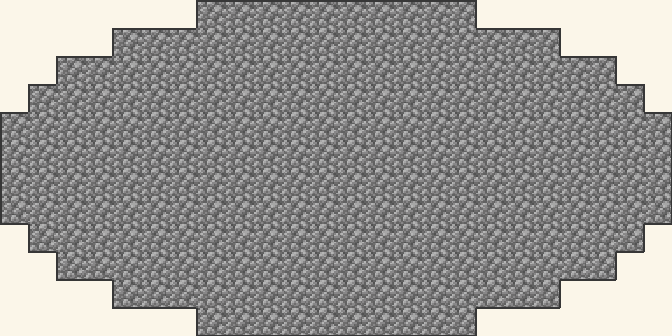
\includegraphics[width=0.45\textwidth]{fig07_2d_ellipse_24x12.png}
\caption{Block Round 中的椭圆 $W = 24, H = 12$。注意长轴方向上的方格分布比短轴方向更"展开"。}
\label{fig:elipse}
\end{figure}

\begin{enumerate}[leftmargin=1.5em,itemsep=0.15em,topsep=0.3em]
  \item 切换形状为 \acc{Ellipse}（椭圆）。出现两个滑杆：\emph{Width} 与 \emph{Height}。
  \item 设 $W = 24$、$H = 12$。观察拉长的形状——见图\ref{fig:elipse}。
  \item 讨论：\emph{"这个图形的方程是 $(x/12)^2 + (y/6)^2 = 1$。为什么 $x$ 除以 12 而 $y$ 除以 6？"}
\end{enumerate}

\subsection{3D 模式、球与椭球}

\begin{enumerate}[leftmargin=1.5em,itemsep=0.15em,topsep=0.3em]
  \item 切换为 \acc{3D / Sphere}，大小 $D = 12$。
  \item 用鼠标拖拽旋转。出现由体素构成的球。
  \item 启用 \emph{Info chip}：记录体积（\emph{"904 blocks $= 14 \times 64 + 8$"}）。
  \item 切到 \acc{Ellipsoid}（椭球），$W = 20$、$H = 10$、$D = 12$。
  \item 演示 Y 轴 \emph{Cut} 滑杆，50\%（见图\ref{fig:cortes}(a)）。观察上半部分消失。
  \item 切到对角 $\swarrow$/$\nearrow$ 轴（$45^\circ$，图\ref{fig:cortes}(c)）。讨论斜切。
\end{enumerate}

\subsection{导出到我的世界}
\begin{enumerate}[leftmargin=1.5em,itemsep=0.15em,topsep=0.3em]
  \item 展示画布角上的\emph{下载}按钮：PNG。
  \item 展示\emph{导出蓝图}按钮：保存为 Sponge v2 格式的 \texttt{.schem} 文件。
  \item 演示（如条件允许）通过 Litematica 模组导入我的世界 Java 版。见附录~\ref{ap:litematica}。
\end{enumerate}

% =============================================================================
\newpage
\section{练习题册}\label{ap:exerc}

\textbf{说明：}独立完成。可在 Block Round 上验证答案，\emph{但数学论证必不可少}。手写或打印提交。

\subsection*{第 1 题 —— 圆的方程}
\textbf{题：}以原点 $(0, 0)$ 为圆心、半径 $r = 7$ 的圆。判断下列每一点在圆\emph{内}、\emph{外}还是\emph{上}。用方程作答。
\begin{enumerate}[label=\alph*),leftmargin=1.5em,itemsep=0.1em,topsep=0.2em,nosep]
  \item $(3, 4)$ \hfill \emph{答案：}内（$9 + 16 = 25 < 49$）。
  \item $(5, 5)$ \hfill \emph{答案：}\acc{外}（$25 + 25 = 50 > 49$, 因为 $\sqrt{50} \approx 7.07$）。
  \item $(0, 7)$ \hfill \emph{答案：}上。
  \item $(-7, 0)$ \hfill \emph{答案：}上。
\end{enumerate}

\textit{教学提示：}(b) 是有意设置的"陷阱"题。

\subsection*{第 2 题 —— stack 与箱子算术}
\textbf{题：}考虑直径 8 的欧几里得圆球，连续体积 $V = \tfrac{4}{3}\pi \cdot 4^3 \approx 268.1$，离散体积 $V_{\mathrm{disc}} = 268$。
\begin{enumerate}[label=\alph*),leftmargin=1.5em,itemsep=0.1em,topsep=0.2em,nosep]
  \item 用圆石建造它需要多少 stack？以 $q$ stack $+$ $r$ 块的形式作答。
  \item 储存所有这些 stack 需要多少单箱（27 格）？
  \item 在生存模式下，若每 0.5 秒挖出一块（铁镐），总采集时间是多少？
\end{enumerate}

\emph{答案：}(a) $268 = 4 \times 64 + 12$，即\acc{4 整 stack $+$ 12 块}（5 个 slot）。(b) 1 个单箱足够（27 格中只用 5 格）。(c) $268 \times 0.5 = 134$ 秒 $\approx$ 2 分 14 秒。

\subsection*{第 3 题 —— D=20 的算法比较}
\textbf{题：}在 Block Round 中生成直径 $D = 20$ 的圆，分别用三种算法。
\begin{enumerate}[label=\alph*),leftmargin=1.5em,itemsep=0.1em,topsep=0.2em,nosep]
  \item 记录每个算法的面积（方块数）。
  \item 哪个算法用料最少？哪个最多？
  \item 最多与最少之间相差几个 stack？为节省材料该选哪个？
\end{enumerate}

\emph{预期答案：}欧几里得约 316 块（4 stack $+$ 60 块），Bresenham 约 316，阈值约 332 块（5 stack $+$ 12 块）。差异：约 1 stack。在更大的项目（$D \geq 32$ 的球）上，差异会累积。

\subsection*{第 4 题 —— 穹顶体积与储存}
\textbf{题：}考虑直径 16 的球，欧几里得算法，Y 轴 50\% 切割（经典穹顶）。
\begin{enumerate}[label=\alph*),leftmargin=1.5em,itemsep=0.1em,topsep=0.2em,nosep]
  \item 整球的连续体积。
  \item 穹顶（上半部）的体积。
  \item 储存穹顶所有方块需要多少双箱？
  \item 还能不能用剩余材料建一层 $16 \times 16$ 的地板？
\end{enumerate}

\emph{答案：}
(a) $V = \tfrac{4}{3}\pi \cdot 8^3 \approx 2\,144.66$，$V_{\mathrm{disc}} \approx 2\,145$。(b) $V_{\mathrm{dome}} \approx 1\,095$。(c) $\lceil 1\,095 / 3\,456 \rceil = 1$ 双箱。(d) 余量：$3\,456 - 1\,095 = 2\,361$ 块。地板 $16 \times 16 = 256$ 块。仍剩 2\,105 块——足够建地板加一层工作台。

\subsection*{第 5 题 —— 椭球"巨型圆桌"}
\textbf{题：}考虑 $W = 24$、$H = 8$、$D = 24$（扁平"圆桌"型）的椭球。
\begin{enumerate}[label=\alph*),leftmargin=1.5em,itemsep=0.1em,topsep=0.2em,nosep]
  \item 连续体积。
  \item Block Round 估计的离散体积。
  \item 如果买了 3 个双箱橡木板，剩多少或缺多少？
\end{enumerate}

\emph{答案：}
(a) $V = \tfrac{4}{3}\pi \cdot 12 \cdot 4 \cdot 12 \approx 2\,413$。
(b) $V_{\mathrm{disc}} \approx 2\,400$（因算法浮动 $\pm 10$）。
(c) 已购容量：$3 \times 3\,456 = 10\,368$ 块。\emph{严重多购}——剩约 8\,000 块。理想是 1 个双箱（剩约 1\,000 块）。

\subsection*{第 6 题 —— WorldEdit vs Block Round}
\textbf{题：}WorldEdit 命令 \cmd{//sphere stone 15} 用类似 Bresenham 3D 的算法。与 Block Round 在 Bresenham 算法、$D = 30$ 下的输出对比：
\begin{enumerate}[label=\alph*),leftmargin=1.5em,itemsep=0.1em,topsep=0.2em,nosep]
  \item 应该完全一致吗？
  \item 若不一致，请列出至少两个原因。
\end{enumerate}

\emph{答案：}
(a) \emph{基本一致}——两者都是 Bresenham 3D，但 (b) 差异原因：(i) 实现差异（Block Round 用 JavaScript，WorldEdit 用 Java）；(ii) 偶/奇直径的中心处理；(iii) 经验性 \emph{threshold} 常数（如果有一方内部用了阈值）。典型差异：$D = 30$ 时相差 0--6 块。

\subsection*{第 7 题 —— 八面体对称建造}
\textbf{题：}规划在 $(0, 72, 0)$ 中心、$D = 16$ 球的我的世界建造，用对称。建一个八分之一象限（$+x, +y, +z$，约 268 块），再用 \cmd{/clone} 反射 7 次。
\begin{enumerate}[label=\alph*),leftmargin=1.5em,itemsep=0.1em,topsep=0.2em,nosep]
  \item 写出 7 条 \cmd{/clone} 命令（用 \cmd{mode:masked} 不覆盖地形）。
  \item 估算总时间：手建八分之一 + 命令执行。
\end{enumerate}

\emph{答案：}

\begin{minecraft}[命令序列]
\cmd{/clone 0 72 0 7 79 7 -8 72 0 mode:masked} \quad （反射 $-x$）\\
\cmd{/clone 0 72 0 7 79 7 0 64 0 mode:masked} \quad\quad （反射 $-y$）\\
\cmd{/clone 0 72 0 7 79 7 0 72 -8 mode:masked} \quad （反射 $-z$）\\
\cmd{/clone -8 72 0 -1 79 7 mode:masked} \quad\quad\;\; （象限 $-x,-y$）\\
\cmd{/clone 0 64 -8 7 71 -1 mode:masked} \quad\quad\;\; （象限 $-y,-z$）\\
\cmd{/clone -8 72 -8 -1 79 -1 mode:masked} \quad\;\; （象限 $-x,-z$）\\
\cmd{/clone -8 64 -8 -1 71 -1 mode:masked} \quad\;\; （象限 $-x,-y,-z$）
\end{minecraft}

时间：约 5 分钟（手建八分之一，生存）+ 约 3 秒（7 次 clone）。

\subsection*{第 8 题 —— 最终项目}
\textbf{题：}完成小组建造（活动~\ref{at:53}）后回答：
\begin{enumerate}[label=(\arabic*),leftmargin=1.7em,itemsep=0.15em,topsep=0.2em,nosep]
  \item 列出用到的几何图形（圆、椭圆、球、椭球）及其参数（直径或半轴）。
  \item 主要图形选用了哪种算法？为什么？它产生了另外两个算法不会产生的什么视觉效果？
  \item 有 3D 切割吗？若有，用不等式描述\emph{其中之一}。
  \item 实际在我的世界生存模式下建造大约需要多少 stack/双箱？
  \item 你们的作品与某种中华文化传统对话吗（古建筑、传统纹样、文人画意、当代艺术、网易我的世界国服建造文化）？请说明。
\end{enumerate}

% =============================================================================
\newpage
\section{无信息技术机房的纸笔版}\label{ap:adapt-analog}

本节适用于当电脑不可用时\emph{完全用纸}实施本序列——这种情形在乡镇普通中学、民族学校（尤其偏远地区）、新疆/西藏/青海/甘肃/宁夏/贵州/云南山区中学，以及一些资源有限的成人高中常见。核心概念脉络不变，仅改变物质支撑。

\subsection{按课分项替代}

\begin{center}
\small
\begin{tabularx}{\textwidth}{@{}p{0.13\textwidth}p{0.32\textwidth}X@{}}
\toprule
\textbf{课次} & \textbf{原活动} & \textbf{纸笔版} \\
\midrule
1 & Block Round 演示（1.3） & 教师在黑板大小的预制网格上手工画出三种 $D = 10$ 圆——每种算法一个。可打印图\ref{fig:comp-d10} 与图\ref{fig:comp-d20} 作参考。\\
\addlinespace[3pt]
2 & 软件中的定量比较（\ref{at:25}） & 分发预先画好的三种 $D = 16$ 圆，要求学生手工计数。\\
\addlinespace[3pt]
3 & 3D 球的生成（\ref{at:31}、\ref{at:32}） & 分发坐标纸上预画好的球\emph{切片}（$z = 0, 1, 2, \ldots$）。学生通过\emph{堆叠}建立心智模型。每张纸代表我的世界中的一\emph{层}。\\
\addlinespace[3pt]
4 & 我的世界命令（\ref{at:42}） & 用书面中文描述的\emph{建造指令}替代命令。学生在坐标纸上模拟执行。\\
\addlinespace[3pt]
5 & 我的世界实战建造（\ref{at:53}） & 用\emph{乐高}（如有），或者在彩色坐标纸上画（用草地绿与泥土棕铅笔），或者用美术课上学生折叠的\emph{纸方块}建造。\\
\bottomrule
\end{tabularx}
\end{center}

\subsection{辅助材料}
完整的纸笔版建议提前准备：
\begin{itemize}[leftmargin=1.3em,itemsep=0.1em,topsep=0.2em,nosep]
  \item 1 张 A3 纸，用直尺画好 $30 \times 30$ 的网格。
  \item 每生 5 张 A4 坐标纸（5\,mm 格）。
  \item 1 张含本计划图\ref{fig:comp-d10} 与图\ref{fig:comp-d20} 三种圆的 A4 印刷对比图作参考。
  \item 第~5~课纸笔版：每组 8 个预折好的纸方块（代表 cobblestone、oak、quartz、diamond 等方块）。
\end{itemize}

\subsection{借助本地传统知识}
在民族中学或工艺传统活跃的地区（藏族唐卡曼陀罗、苗族银饰、新疆维吾尔族花毯、贵州苗族刺绣、福建客家土楼工匠、内蒙古蒙古包毡匠、广西壮族织锦、景德镇陶瓷拉坯），\emph{第~\ref{aula3}~课可邀请本地传统手艺人到课堂}：让他们展示自己如何在不同的材料语言中"光栅化"圆形或对称图案。此举既落实了民族数学的精神，也呼应了《民族区域自治法》与课程标准关于文化认同的要求。

% =============================================================================
\newpage
\section{教师用术语表}\label{ap:glos}

\begin{itemize}[leftmargin=1.4em,itemsep=0.3em,topsep=0.3em]
  \item \acc{算法} —— 解决问题的有限、明确的指令序列。Block Round 的三种算法（参见图\ref{fig:comp-d10}）是同一问题的三种不同程序。
  \item \acc{单箱} —— 我的世界中 27 格的存储容器。容量：$27 \times 64 = 1\,728$ 件。
  \item \acc{双箱} —— 两个相邻的箱子合并为 54 格的容器。容量：$54 \times 64 = 3\,456$ 件。
  \item \acc{方块} —— 我的世界的基本构造单位。带六面贴图的 $1 \times 1 \times 1$ 立方体。在数学语言中即\emph{体素}。
  \item \acc{Bresenham 算法} —— Jack Bresenham 1965 年在 IBM 发表的整数光栅化算法，原本用于直线，后由 Pitteway（1967）等人推广到椭圆。其标志是\emph{只用整数运算}。见活动~\ref{at:23}。
  \item \acc{课标} —— 中华人民共和国教育部颁发的课程标准。本序列对接《普通高中数学课程标准（2017年版2020年修订）》。
  \item \acc{Canvas} —— HTML 元素，在浏览器中提供 2D 或 3D 绘图空间。
  \item \acc{\code{/clone}} —— 我的世界原版命令，把一个矩形区域复制到另一位置。语法：\cmd{/clone x1 y1 z1 x2 y2 z2 dx dy dz}。对称建造的关键。
  \item \acc{高考} —— 普通高等学校招生全国统一考试。
  \item \acc{隐式方程} —— 形如 $F(x, y) = 0$ 的方程。椭圆的隐式方程：$(x/r_x)^2 + (y/r_y)^2 - 1 = 0$。
  \item \acc{民族数学（ethnomathematics）} —— 由乌比拉坦·杜安布罗西奥（D'Ambrosio）创立的研究领域，中国学者张维忠等做了系统译介。
  \item \acc{\code{/fill}} —— 我的世界原版命令，把矩形盒填满某种方块。语法：\cmd{/fill x1 y1 z1 x2 y2 z2 minecraft:stone}。
  \item \acc{AMSS-CAS} —— 中国科学院数学与系统科学研究院。
  \item \acc{BICMR} —— 北京国际数学研究中心（北京大学）。
  \item \acc{YMSC} —— 清华大学丘成桐数学科学中心。
  \item \acc{PIPL} —— 《个人信息保护法》。
  \item \acc{Litematica} —— 我的世界 Java 版的流行模组，导入蓝图后显示半透明"幽灵"建筑，逐块指导建造。免费。
  \item \acc{Minecraft Education} —— 我的世界教育版。在中国大陆通过网易我的世界国服发行。
  \item \acc{NOIP/NOI} —— 全国青少年信息学奥林匹克联赛/竞赛。由中国计算机学会（CCF）组织。
  \item \acc{Pack / Stack} —— 我的世界物品栏一格中最多 64 块同种方块的堆叠。
  \item \acc{Pixel} —— picture element 的缩写，2D 的像素。
  \item \acc{PWA} —— Progressive Web App（渐进式网页应用），可安装、可离线运行的网页应用。
  \item \acc{光栅化（rasterization）} —— 把连续几何描述转化为像素矩阵（2D）或体素矩阵（3D）的过程。
  \item \acc{Schematica} —— Litematica 的替代模组，功能类似。
  \item \acc{Schematic (\texttt{.schem})} —— 序列化我的世界区域的文件格式（Sponge Schematic v2，gzip + NBT）。
  \item \acc{半轴} —— 椭圆中，从圆心到长/短轴端点的距离。
  \item \acc{\code{//sphere}} —— WorldEdit 模组中绘制球的命令。语法：\cmd{//sphere block radius}。
  \item \acc{Slot} —— 我的世界物品栏的单个格子。玩家完整物品栏：36 格（$9 \times 4$）。
  \item \acc{体素（voxel）} —— volume element 的缩写。pixel 在 3D 的推广。在我的世界中每块方块即一个体素。
  \item \acc{WebGL} —— 浏览器中的 3D 图形编程库。
  \item \acc{WorldEdit} —— 我的世界 Java 版非常流行的模组，提供大规模建造命令，包括 \cmd{//sphere}、\cmd{//hsphere}、\cmd{//ellipsoid}、\cmd{//cyl}、\cmd{//schem load}。
\end{itemize}

% =============================================================================
\newpage
\section{教程：从 Block Round 到我的世界（通过 Litematica）}\label{ap:litematica}

本附录描述 Block Round 导出 + 我的世界 Java 版 Litematica 模组导入的完整流程。预计总时间：15 分钟（首次）。

\subsection{前置条件}
\begin{itemize}[leftmargin=1.3em,itemsep=0.1em,topsep=0.2em,nosep]
  \item 我的世界 Java 版（在 Mojang 商店购买；教育版 Minecraft Education 经过调整也可使用；中国大陆地区也可使用网易我的世界国服）。
  \item 与你使用的我的世界版本匹配的 \emph{Fabric Loader}（一般取最新：\url{https://fabricmc.net/use/}）。
  \item 模组：\emph{Fabric API} 与 \emph{Litematica}（\url{https://www.curseforge.com/minecraft/mc-mods/litematica}）。
  \item 在浏览器中打开 Block Round 并已生成目标图形。
\end{itemize}

\subsection{步骤 1：从 Block Round 导出}
\begin{enumerate}[leftmargin=1.5em,itemsep=0.15em,topsep=0.3em]
  \item 在 Block Round 中配置目标图形（模式、形状、直径、算法、方块、切割）。在 \emph{Info chip} 中核对体积。
  \item 点击画布右上角第二个图标 \emph{Export Schematic}。一个 \texttt{.schem} 文件会被下载。
\end{enumerate}

\subsection{步骤 2：安装 Litematica}
\begin{enumerate}[leftmargin=1.5em,itemsep=0.15em,topsep=0.3em]
  \item 为你使用的我的世界版本安装 Fabric Loader。
  \item 为同一我的世界版本下载 \emph{Fabric API} 与 \emph{Litematica}，把两者放进 \texttt{.minecraft/mods/} 目录。
  \item 用 \emph{fabric-loader-x.y.z-1.20.x} 配置启动我的世界。
\end{enumerate}

\subsection{步骤 3：导入蓝图}
\begin{enumerate}[leftmargin=1.5em,itemsep=0.15em,topsep=0.3em]
  \item 把 \texttt{.schem} 文件放入 \texttt{.minecraft/schematics/}（或 Litematica 设置中指定的默认文件夹）。
  \item 在一个世界（创造或生存）中，按 \texttt{M} 打开 Litematica 菜单。
  \item 点击 \emph{Load Schematic} $\to$ 选择文件 $\to$ \emph{Load}。
  \item 蓝图出现在列表中。点选它再点 \emph{Placement}：半透明的"幽灵"出现在世界中。
  \item 用移动控件（\texttt{M} $\to$ \emph{Placements}）把"幽灵"拖到目标位置。地面平整的话，把 $(x_1, y_1, z_1)$ 放在地面即可。
\end{enumerate}

\subsection{步骤 4：建造}
\begin{enumerate}[leftmargin=1.5em,itemsep=0.15em,topsep=0.3em]
  \item \emph{创造模式}：在"幽灵"上方飞行，按 Litematica 指示放置每块方块；正确方块被标记为绿色，错位标记为红色。一个 $D = 12$ 球大约 5 分钟。
  \item \emph{生存模式}：流程相同，但需先采集方块。用活动~\ref{at:41} 的 stack/双箱算式规划采集。
  \item 替代方案：若服务器有 WorldEdit，使用 \cmd{//schem load filename} 后 \cmd{//paste -a} 实现即时建造。
\end{enumerate}

\subsection{步骤 5：校验}
Litematica 用红色高亮任何错误（缺失、错类型、错位置）的方块。用快捷键 \texttt{Z} 切换"幽灵"的可见与不可见，便于对照真实建造。

\subsection{常见问题排查}
\begin{itemize}[leftmargin=1.3em,itemsep=0.15em,topsep=0.3em,nosep]
  \item \emph{蓝图不在列表中：}检查文件位置；检查 Litematica 与我的世界版本是否兼容。
  \item \emph{方块错误/灰色：}Block Round 蓝图中的某些方块可能在你的版本中不可用（旧版本我的世界）；用文本编辑器查看蓝图的方块名称。
  \item \emph{幽灵悬空：}在 Placement 菜单调整 \emph{Rotation/Mirror}。对球而言无关紧要；对椭圆需调整旋转。
\end{itemize}

\vspace{2em}
\begin{center}
\color{muted}\small\sffamily
--- 教学设计完 ---
\end{center}

\end{document}
